%% LyX 2.0.1 created this file.  For more info, see http://www.lyx.org/.
%% Do not edit unless you really know what you are doing.
\documentclass[english]{beamer}
\usepackage[T1]{fontenc}
\usepackage[latin9]{inputenc}
% \usepackage[usenames,dvipsnames]{xcolor}
\setcounter{secnumdepth}{3}
\setcounter{tocdepth}{3}
\usepackage{verbatim}
\usepackage{float}
\usepackage{amsthm}
\usepackage{amsmath}
\usepackage{graphicx}

\usepackage{libertine}
\usepackage{caption}
\usepackage{subcaption}
\captionsetup[subfigure]{labelformat=empty}

%% for manually breaking cells in tables.
\newcommand{\specialcell}[2][c]{%
  \begin{tabular}[#1]{@{}c@{}}#2\end{tabular}}

  %%%%
\usepackage{booktabs}
\newcommand{\ra}[1]{\renewcommand{\arraystretch}{#1}}



\newcommand{\tgemmcpu}{\ensuremath{t_{\mbox{\tiny\scshape Gemm}}}\xspace}
\newcommand{\tscattercpu}{\ensuremath{t_{\mbox{\tiny\scshape Scatter}}}\xspace}
\newcommand{\tgemmmic}{\ensuremath{t_{\mbox{\tiny\scshape Gemm}}^{\tiny (\phi)}}\xspace}
\newcommand{\tscattermic}{\ensuremath{t_{\mbox{\tiny\scshape Scatter}}^{\tiny (\phi)}}\xspace}

\newcommand{\bigNotation}[2]{\ensuremath{\operatorname{#1}\bigl({#2}\bigr)}}
\newcommand{\bigO}[1]{\bigNotation{\mathcal{O}}{#1}}
\newcommand{\littleO}[1]{\bigNotation{\mathcal{o}}{#1}}
\newcommand{\bigOmega}[1]{\bigNotation{\Omega}{#1}}
\newcommand{\bigTheta}[1]{\bigNotation{\Theta}{#1}}


%% defenitions for different colrs 
% Dark pastel green
\definecolor{dpg}{rgb}{0.01, 0.75, 0.24}
\definecolor{emerald}{rgb}{0.31, 0.78, 0.47}

\usepackage{eso-pic}
\beamertemplatenavigationsymbolsempty
\setbeamertemplate{footline}[frame number]

\newcommand\AtPagemyUpperLeft[1]{\AtPageLowerLeft{%
\put(\LenToUnit{0.6\paperwidth},\LenToUnit{0.97\paperheight}){#1}}}
\AddToShipoutPictureFG{
  \AtPagemyUpperLeft{http://hpcgarage.org/ftxs16/}
}%

\makeatletter

%%%%%%%%%%%%%%%%%%%%%%%%%%%%%% LyX specific LaTeX commands.
%% A simple dot to overcome graphicx limitations
\newcommand{\lyxdot}{.}
% \newcommand{\comment}[1]{}


%%%%%%%%%%%%%%%%%%%%%%%%%%%%%% Textclass specific LaTeX commands.
 % this default might be overridden by plain title style
 \newcommand\makebeamertitle{\frame{\maketitle}}%
 \AtBeginDocument{
   \let\origtableofcontents=\tableofcontents
   \def\tableofcontents{\@ifnextchar[{\origtableofcontents}{\gobbletableofcontents}}
   \def\gobbletableofcontents#1{\origtableofcontents}
 }
 \long\def\lyxframe#1{\@lyxframe#1\@lyxframestop}%
 \def\@lyxframe{\@ifnextchar<{\@@lyxframe}{\@@lyxframe<*>}}%
 \def\@@lyxframe<#1>{\@ifnextchar[{\@@@lyxframe<#1>}{\@@@lyxframe<#1>[]}}
 \def\@@@lyxframe<#1>[{\@ifnextchar<{\@@@@@lyxframe<#1>[}{\@@@@lyxframe<#1>[<*>][}}
 \def\@@@@@lyxframe<#1>[#2]{\@ifnextchar[{\@@@@lyxframe<#1>[#2]}{\@@@@lyxframe<#1>[#2][]}}
 \long\def\@@@@lyxframe<#1>[#2][#3]#4\@lyxframestop#5\lyxframeend{%
   \frame<#1>[#2][#3]{\frametitle{#4}#5}}
 \def\lyxframeend{} % In case there is a superfluous frame end

%%%%%%%%%%%%%%%%%%%%%%%%%%%%%% User specified LaTeX commands.

\usepackage{listings}
%\usetheme{Warsaw}
% or ...
%\usetheme{Antibes}	% tree outline, neat
%\usetheme{JuanLesPins}	% like Antibes, with shading
%\usetheme{Bergen}	% outline on side
%\usetheme{Luebeck}	% like Warsaw, square sides
%\usetheme{Berkeley}	% interesting left bar outline
\usetheme{CambridgeUS}  
% \usetheme{Madrid}	% clean, nice.  7/12 page numbers
%\usetheme{Berlin}	% dots show slide number
%\usetheme{Malmoe}	% OK, plain, unshaded
%\usetheme{Boadilla}	% nice, white bg, no top bar
%\usetheme{Marburg}	% nice, outline on right
%\usetheme{boxes}	% ???
%\usetheme{Montpellier}	% tree outline on top, plainish white
%\usetheme{Copenhagen}	% like Warsaw
% \usetheme{PaloAlto}	% looks good
%\usetheme{Darmstadt}	% like Warsaw with circle outline
% \usetheme{Pittsburgh}
% \usetheme{default}
%\usetheme{Rochester}	% like boxy, unshaded warsaw
%\usetheme{Dresden}	% circle outline on top
%\usetheme{Singapore}	% purple gradient top
%\usetheme{Frankfurt}	% like Warsaw with circle outline on top
%\usetheme{Szeged}
%\usetheme{Goettingen}	% light purple right bar outline
% \usetheme{Warsaw}
%\usetheme{Hannover}	% like Goett with bar on left
%\usetheme{compatibility}
%\usetheme{Ilmenau}

\setbeamertemplate{footline}
{
  \leavevmode%
  \hbox{%
  \begin{beamercolorbox}[wd=.333333\paperwidth,ht=2.25ex,dp=1ex,center]{author in head/foot}%
    \usebeamerfont{author in head/foot}\insertshortauthor~~\beamer@ifempty{\insertshortinstitute}{}{\insertshortinstitute}
  \end{beamercolorbox}%
  \begin{beamercolorbox}[wd=.333333\paperwidth,ht=2.25ex,dp=1ex,center]{title in head/foot}%
    \usebeamerfont{title in head/foot}\insertshorttitle
  \end{beamercolorbox}%
  \begin{beamercolorbox}[wd=.333333\paperwidth,ht=2.25ex,dp=1ex,right]{date in head/foot}%
    \usebeamerfont{date in head/foot}\insertshortdate{}\hspace*{2em}
    \insertframenumber{} / \inserttotalframenumber\hspace*{2ex} 
  \end{beamercolorbox}}%
  \vskip0pt%
}

\setbeamercovered{transparent}
% or whatever (possibly just delete it)

% \usecolortheme{seahorse}
\usecolortheme{rose}
% \usecolortheme{beaver}

% seems to fix typewriter font in outline header:
\usepackage{ae,aecompl}


%%%
\newenvironment<>{problock}[1]{%
  \begin{actionenv}#2%
      \def\insertblocktitle{#1}%
      \par%
      \mode<presentation>{%
        \setbeamercolor{block title}{fg=white,bg=YellowGreen}
       \setbeamercolor{block body}{fg=black,bg=olive!50}
       \setbeamercolor{itemize item}{fg=orange!20!black}
       \setbeamertemplate{itemize item}[triangle]
     }%
      \usebeamertemplate{block begin}}
    {\par\usebeamertemplate{block end}\end{actionenv}}




\makeatother

\usepackage{babel}
\begin{document}

\title[Fault tolerant graph computing]{A Self-correcting Graph Connected Component Algorithm}


\author[Piyush Sao]{\underline{Piyush Sao}, Oded Green, Chirag Jain, Richard Vuduc}

\date[FTXS16]{ The $6^{th}$ Workshop on Fault Tolerance for HPC at eXtreme Scale (FTXS) 2016\\ \url{http://hpcgarage.org/ftxs16/}}
% \institute{CSE}

\titlegraphic{

\includegraphics[width=4cm]{logo/cse}\hspace*{.5cm}~

\includegraphics[width=3.5cm]{logo/HPClogo_rgb}
}

\makebeamertitle

% \lyxframe{Outline of talk}
% \tableofcontents{}
% \lyxframeend{}

\fontsize{9pt}{11}\selectfont
\section{Summary}
\lyxframe{Summary of Contributions }

\begin{alertblock}{Self-correcting Algorithms}

We introduce a new fault tolerant algorithm design principle that we call \emph{self-correction}. A self-correcting algorithm remains in a valid state, despite the faulty execution of an iteration, under the assumption that its previous state was a valid one. 
\end{alertblock}
\pause
\begin{exampleblock}{Self-Correcting Connected Components Algorithm}
\begin{itemize}
\item We apply the ideas of self-correction to Label-propagation algorithm for graph connected component problem.
\item Assumes availability of selective reliability mode.
\item Requires $\bigO{V}$ additional storage and computations per iteration compared to $\bigO{|V|+|E|}$ cost for the baseline algorithm.
\item 10-35\%  increases in execution time for one error for 64 memory operations.
\end{itemize}
\end{exampleblock}

\lyxframeend{}

\section{Self-correcting Algorithms}
\lyxframe{Iterative Algorithms}
\begin{columns}
\begin{column}{0.4\textwidth}
\only<1>{
\centering
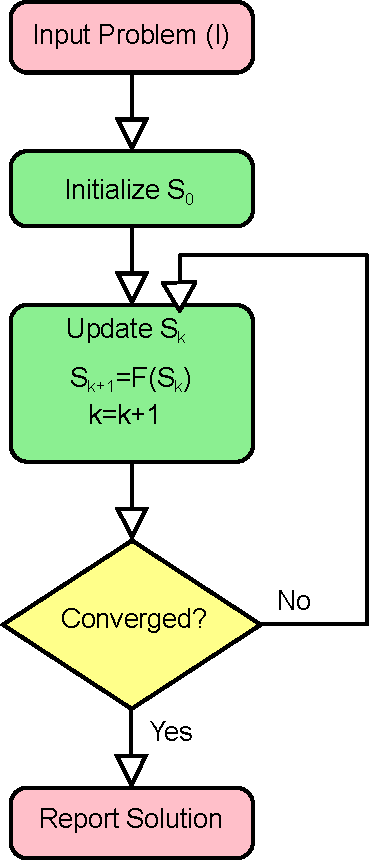
\includegraphics[height=0.8\textheight]{images/iterative-algm}

}

\end{column}
\begin{column}{0.6\textwidth}
\begin{block}{Iterative Algorithms}
\begin{itemize}
\item A typical iterative algorithm has following components:
\begin{enumerate}
\item The input problem;
\item Intermediate variable; 
\item Update relation; 
\item Convergence checking; and 
\item Solution. 
\end{enumerate}
\end{itemize}
\end{block}
\end{column}

\end{columns}

\lyxframeend{}

%%%%%%%%%%%%%%%%%%%%%%%%%%%%%%%%%%%%%%%%%%%%%%%%%%%%%%%%%
\lyxframe{Iterative Algorithm as State Machine}
\begin{columns}
\begin{column}{0.4\textwidth}
\only<1>{
\centering
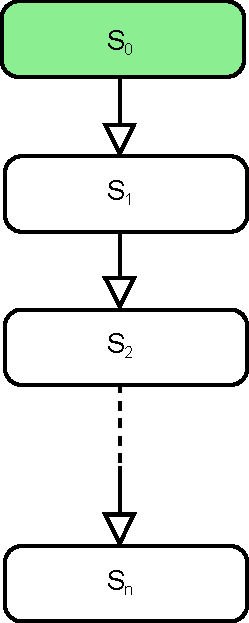
\includegraphics[height=0.8\textheight]{images/iterative-sm/iterative-sm-1}

}
\only<2>{
\centering
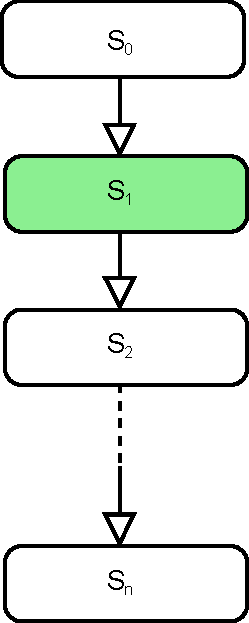
\includegraphics[height=0.8\textheight]{images/iterative-sm/iterative-sm-2}

}
\only<3>{
\centering
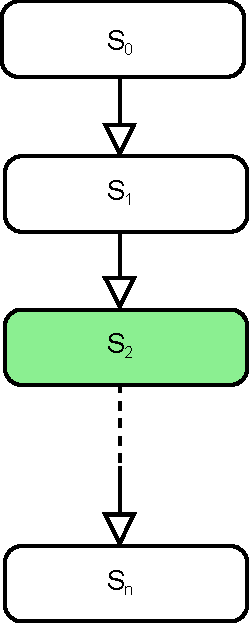
\includegraphics[height=0.8\textheight]{images/iterative-sm/iterative-sm-3}

}
\only<4>{
\centering
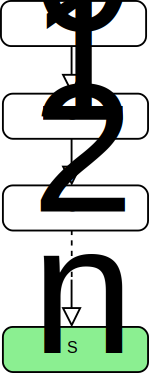
\includegraphics[height=0.8\textheight]{images/iterative-sm/iterative-sm-4}

}


\end{column}
\begin{column}{0.6\textwidth}
\begin{block}{Iterative Algorithms as State Machines}
\begin{itemize}
\item An iterative algorithm can be viewed as state machine.
\item State of the algorithm: subset of intermediate variables required for continued execution of the algorithm.
\item Starts with an initial state $S_{0}$
\item Uses update relation to transition from one state to another 
\[
S_{k+1} \leftarrow S_{k}
\]
\end{itemize}
\end{block}
\end{column}
\end{columns}

\lyxframeend{}

%%%%%%%%%%%%%%%%%%%%%%%%%%%%%%%%%%%%%%%%%%%%%%%%%%%%%%%%%
\lyxframe{Single Fault in Iterative Algorithm}
\begin{columns}
\begin{column}{0.5\textwidth}
\only<1>{
\centering
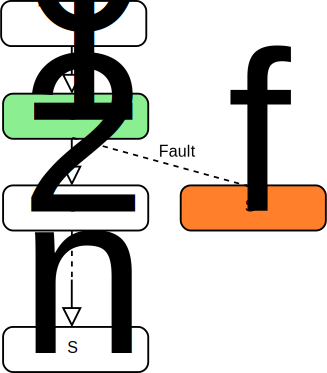
\includegraphics[height=0.6\textheight]{images/iterative-fault}

}
\only<2>{
\centering
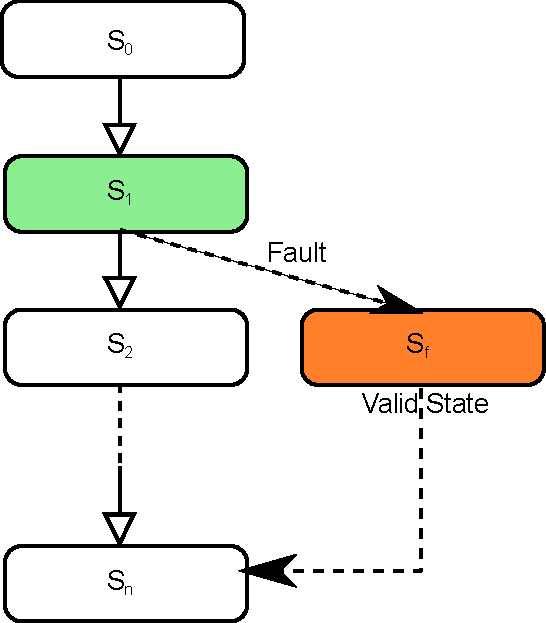
\includegraphics[height=0.6\textheight]{images/iterative-valid}

}
\only<3>{
\centering
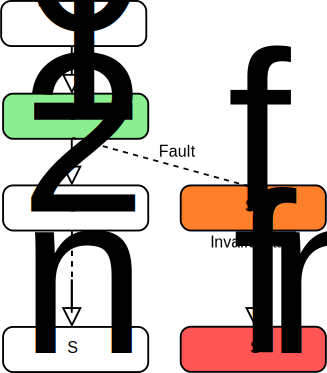
\includegraphics[height=0.6\textheight]{images/iterative-invalid}

}
\end{column}
\begin{column}{0.5\textwidth}
\begin{block}{Valid and Invalid States}

\begin{itemize}
\item Valid state: under fault-free execution of the algorithm from that state, the algorithm will converge to the correct solution; otherwise invalid. 
\item In fault free execution, the algorithm always remains in a valid state.
\item Any hardware fault can cause the algorithm to reach an invalid state.
\item In general determining whether a given state is valid or not, is non-trivial.     
\end{itemize}
\end{block}
\end{column}
\end{columns}


\lyxframeend{}

%%%%%%%%%%%%%%%%%%%%%%%%%%%%%%%%%%%%%%%%%%%%%%%%%%%%%%%%%
\lyxframe{Self-stabilizing Algorithms}
\begin{columns}
\begin{column}{0.5\textwidth}
\only<1>{
\centering
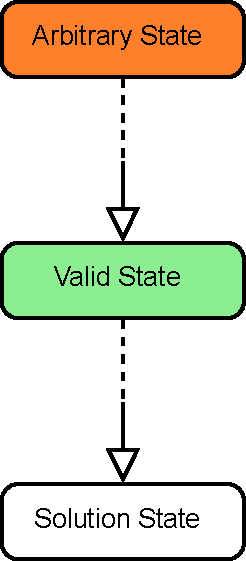
\includegraphics[height=0.6\textheight]{images/self-stab}

}

\end{column}
\begin{column}{0.5\textwidth}
\begin{block}{Self-stabilizing Algorithms}
\begin{itemize}
\item Starting from any arbitrary state, valid or invalid, a self-stabilizing algorithm will reach a valid in finite number of steps. 
\item Natural fault-tolerance mechanism.
\item Examples: Stationary iterations, Newton Iteration. 
\item Self-stabilization is a \emph{strong} property.
%, as it does not assume any thing about history of computation.
\end{itemize}
\end{block}

\begin{block}{Scala'13}
\begin{itemize}
\item Self-stabilizing Steepest Descent and Conjugate Gradient.
\item Periodic state correction.
\item May not be generalized to all iterative algorithms.
\end{itemize}
\end{block}
\end{column}
\end{columns}

\lyxframeend{}

%%%%%%%%%%%%%%%%%%%%%%%%%%%%%%%%%%%%%%%%%%%%%%%%%%%%%%%%%
\lyxframe{Self-Correcting Algorithms}
\begin{columns}
\begin{column}{0.5\textwidth}
\only<1>{
\centering
\includegraphics[height=0.6\textheight]{images/self-correction}

}

\end{column}
\begin{column}{0.5\textwidth}
\begin{block}{Self-correcting Algorithms}
\begin{itemize}
\item A self-correcting algorithm is an iterative algorithm that, starting in some valid state, remains in a valid state or comes to a valid state in finite number of steps even if a fault occurs.
\item Requires that algorithm starts from a valid state. 
\item Uses information from previously known valid state.
% to detect invalid states, or to bring it to a valid state.
\item Example: Checkpoint-restart, FT-GMRES. 

\end{itemize}
\end{block}
\end{column}
\end{columns}


\lyxframeend{}

%%%%%%%%%%%%%%%%%%%%%%%%%%%%%%%%%%%%%%%%%%%%%%%%%%%%%%%%%
\lyxframe{Checkpoint-restart as a Self-correcting algorithm}
\begin{columns}
\begin{column}{0.5\textwidth}
\only<1>{
\centering
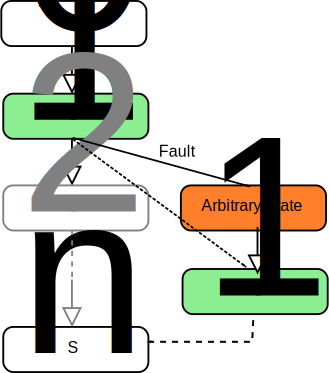
\includegraphics[height=0.6\textheight]{images/checkpt-restart}

}
\only<2>{
\centering
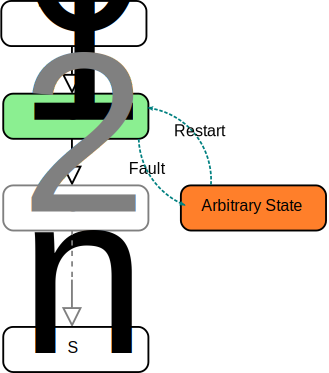
\includegraphics[height=0.6\textheight]{images/checkpt-restart-1}

}
\only<3>{
\centering
\includegraphics[height=0.6\textheight]{images/self-correction-1}

}

\end{column}
\begin{column}{0.5\textwidth}
\begin{block}{Checkpoint-restart based fault tolerance}
\begin{itemize}
\item<1-> Bring to valid state by restoring a check-pointed valid state.
\item<2-> \color{red} At high fault rate, algorithm will not make any progress.



\end{itemize}
\end{block}

\pause
\pause
{\color{dpg} Broader idea of self-correction is to use $S_{1}$ to construct an state 
\[\tilde{S}_{2} \approx S_{2}
\]
}
\end{column}
\end{columns}


\lyxframeend{}

\section{Self-correcting Label-propagation Algorithm}
\lyxframe{Label Propagation Algorithm for Graph Connected Component Algorithm}

\only<1>{
\centering
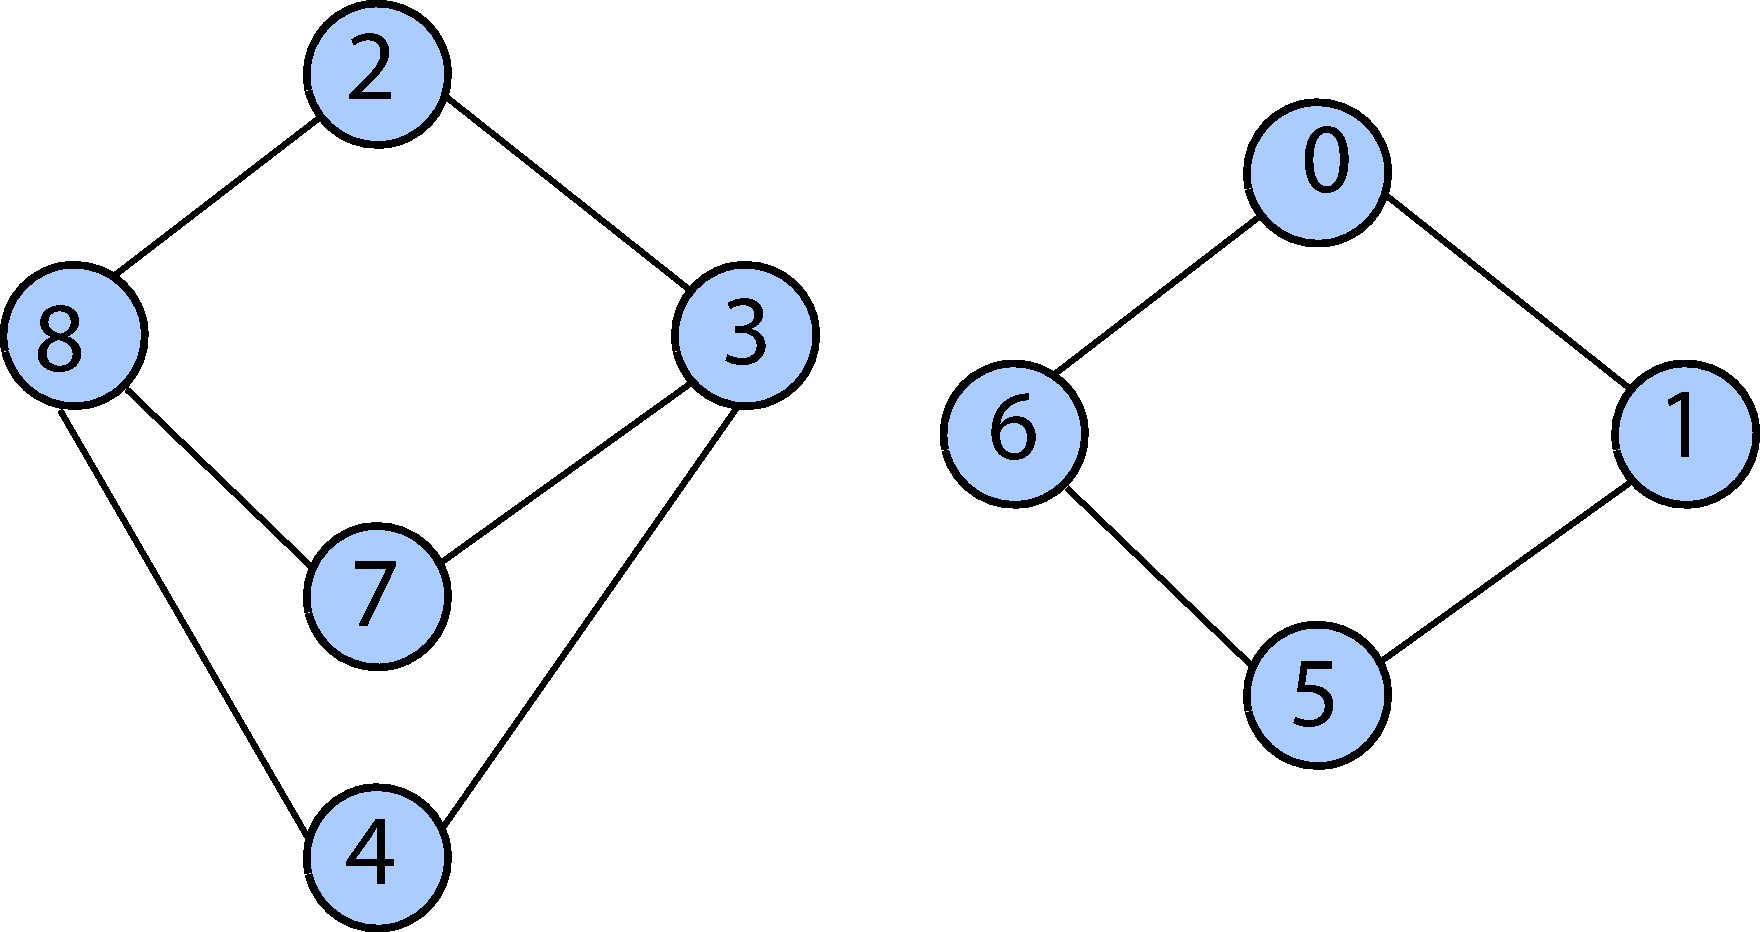
\includegraphics[height=0.4\textheight]{images/base}
}
\only<2>{
\centering
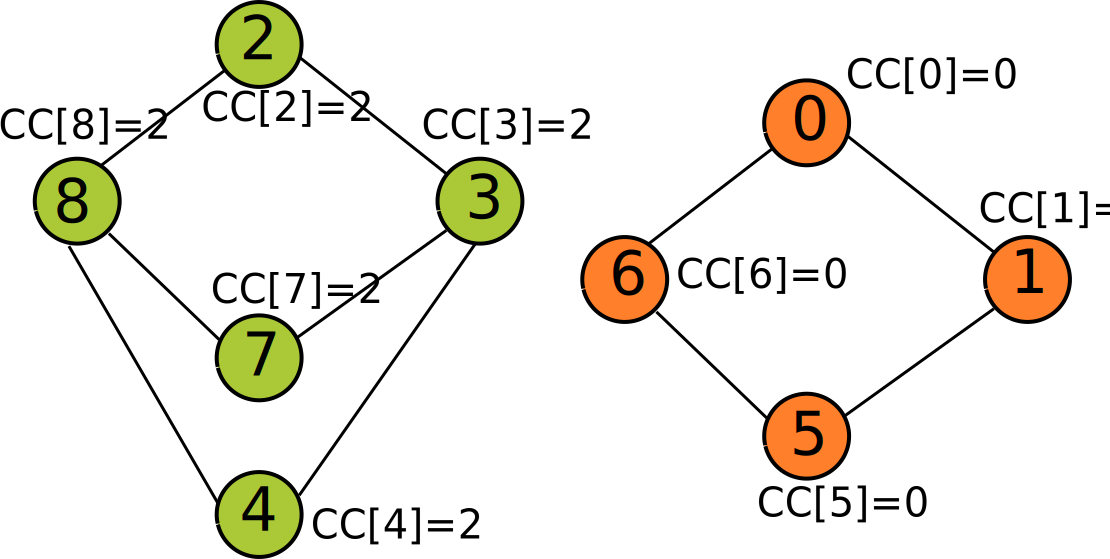
\includegraphics[height=0.4\textheight]{images/lp/lp-4}
}

\begin{block}{Graph Connected-component Problem}
We seek to find number of connected-components in the graph and which connected component 
each vertex belongs to.
\begin{itemize}
\item Used for community detection, centrality analytics and streaming graph analytics. 
\item Label propagation is highly suited for parallel computing. 
\end{itemize}
\end{block}
\lyxframeend{}
%%%%%%%%%%%%%%%%%%%%%%%%%%%%%%%%%%%%%%%%%%%%%%%%%%%%%%%%%
\lyxframe{Label Propagation Algorithm}

\only<1>{
\centering
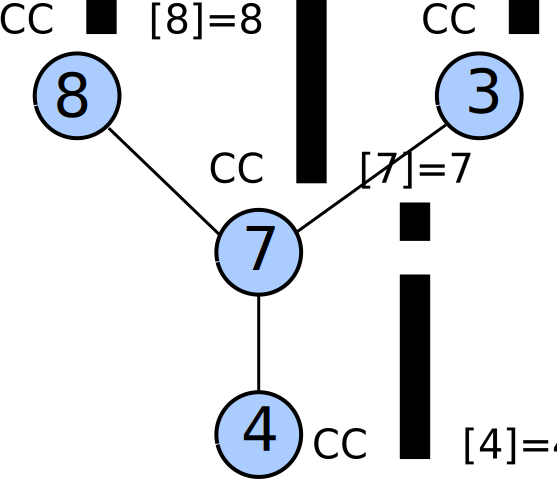
\includegraphics[height=0.4\textheight]{images/lp-initialize}

}
\only<2>{
\centering
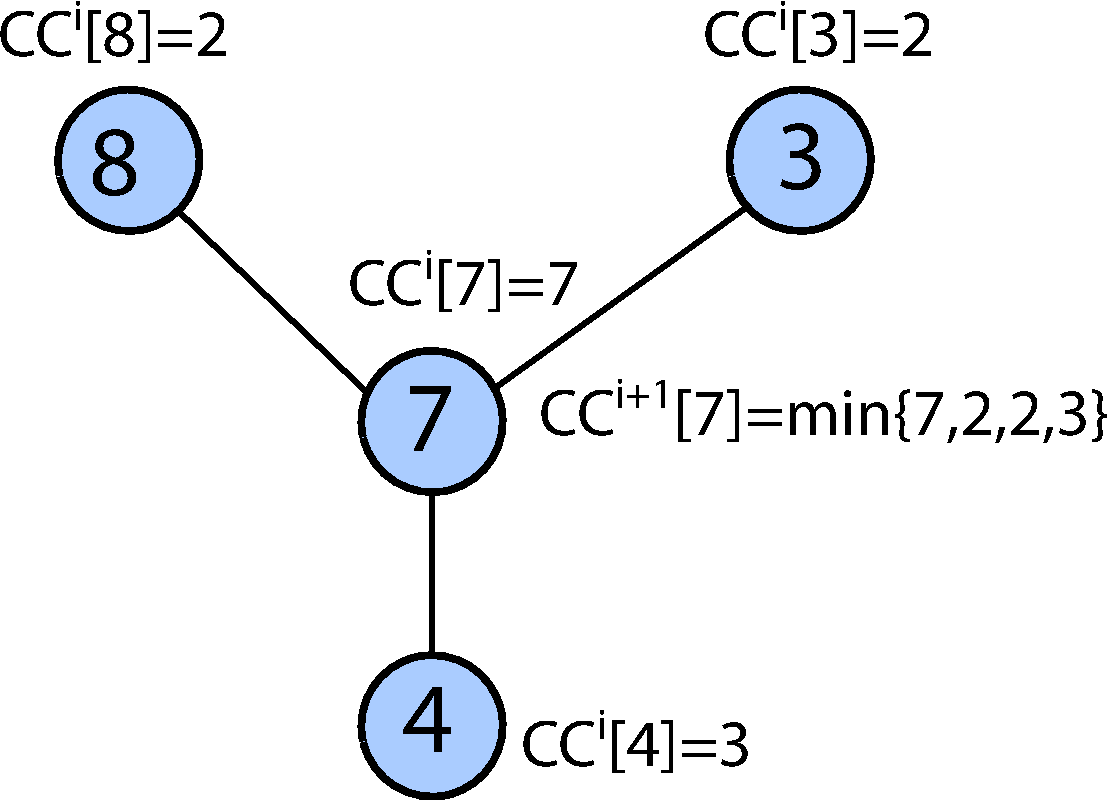
\includegraphics[height=0.4\textheight]{images/lp-update}

}


\begin{itemize}
\item Propagates the minimum label in the connected component.
\item We maintain a \emph{label} array $CC$ for each vertex.
\item $CC$ is initialized to vertex id for each vertex.
\item In each iteration, each vertex calculates minimum label among all near-neighbours $\mathcal{N}(v)=v\cup adj(v)$
\[ CC^{i}[v] = \min_{u \in \mathcal{N}(v)} CC^{i-1}[u]. \]
\item Iteration terminates when no change occur in an iteration.

\end{itemize}
\lyxframeend{}

%%%%%%%%%%%%%%%%%%%%%%%%%%%%%%%%%%%%%%%%%%%%%%%%%%%%%%%%%
\lyxframe{Label Propagation Algorithm- Example}

\only<1>{
\centering
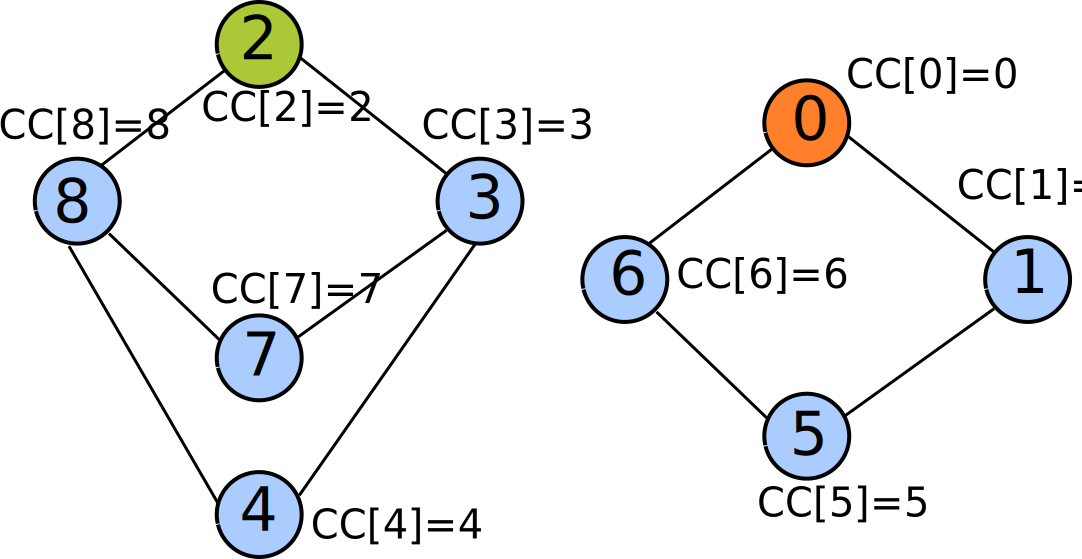
\includegraphics[height=0.4\textheight]{images/lp/lp-1}

}
\only<2>{
\centering
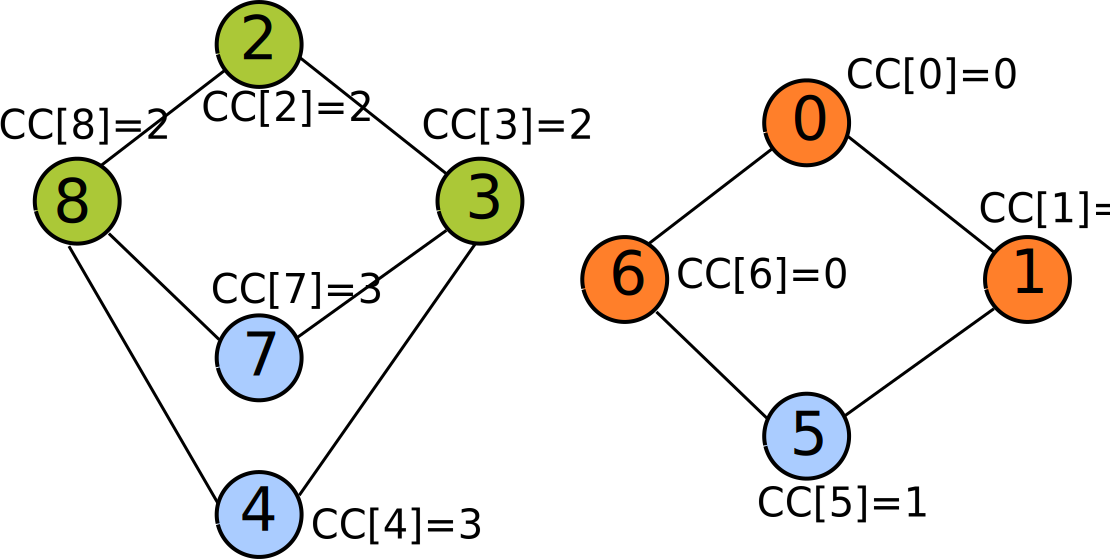
\includegraphics[height=0.4\textheight]{images/lp/lp-2}

}
\only<3>{
\centering
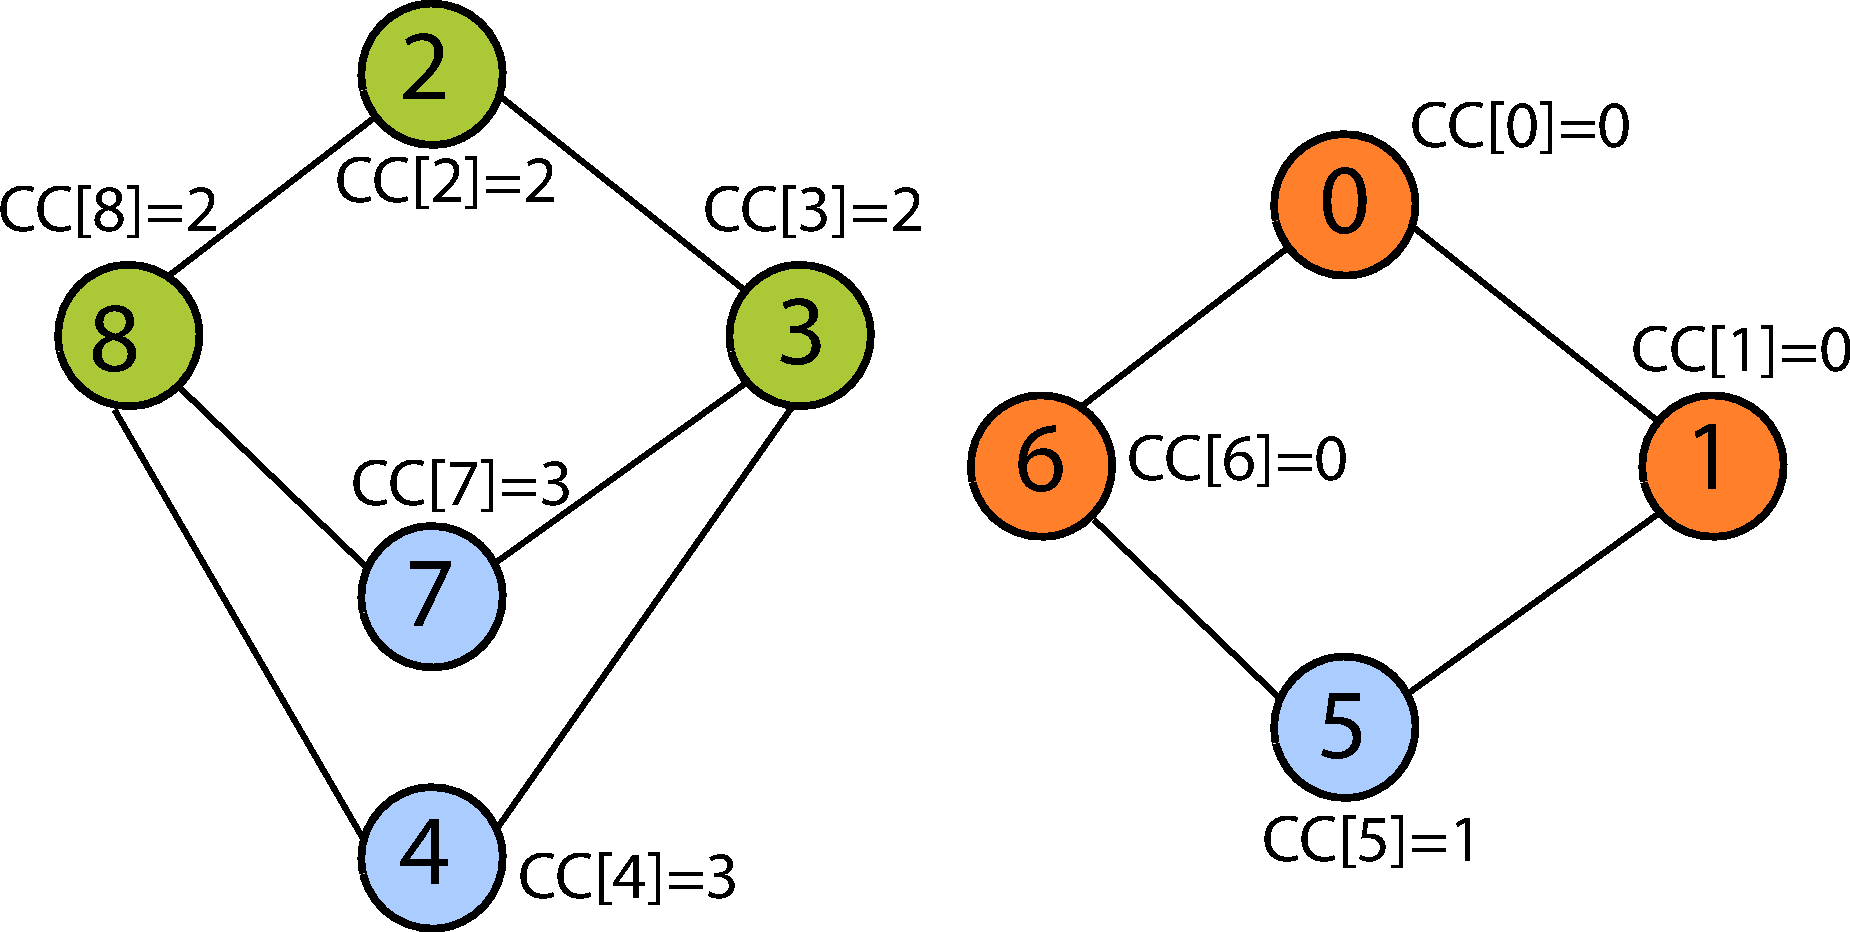
\includegraphics[height=0.4\textheight]{images/lp/lp-3}

}
\only<4>{
\centering
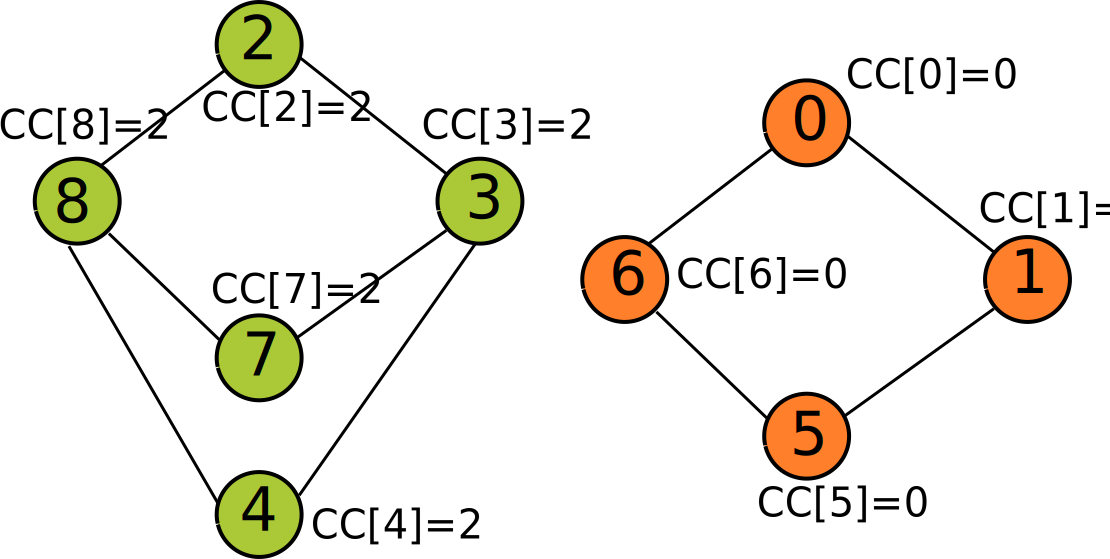
\includegraphics[height=0.4\textheight]{images/lp/lp-4}

}

\begin{itemize}
\item Minimum label in the connected component (shown in {\color{green} green} and {\color{orange} orange} ) propagates to all the vertex in the connected components. 
\end{itemize}
\lyxframeend{}

%%%%%%%%%%%%%%%%%%%%%%%%%%%%%%%%%%%%%%%%%%%%%%%%%%%%%%%%%
\lyxframe{State of Label Propagation Algorithm}
\begin{columns}
% change following images
\begin{column}{0.5\textwidth}  %%<--- here
    \only<1>{
\centering
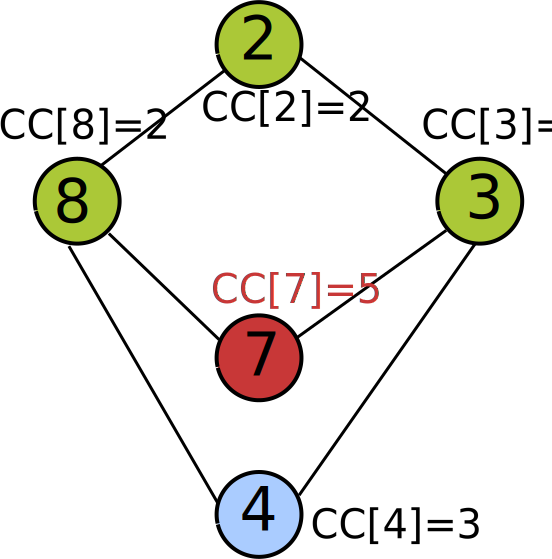
\includegraphics[height=0.5\textheight]{images/fault-corrected/fault-corrected-1}

}

\end{column}

\begin{column}{0.5\textwidth}
   \begin{itemize}
   \item<1-> $CC$ vector defines the state of the LP algorithm.
   
   \end{itemize}
\end{column}

\end{columns}


\lyxframeend{}

%%%%%%%%%%%%%%%%%%%%%%%%%%%%%%%%%%%%%%%%%%%%%%%%%%%%%%%%%
\lyxframe{Single Fault In Label Propagation Algorithm- Fault Correction}
\begin{columns}
\begin{column}{0.5\textwidth}

\only<1>{
\centering
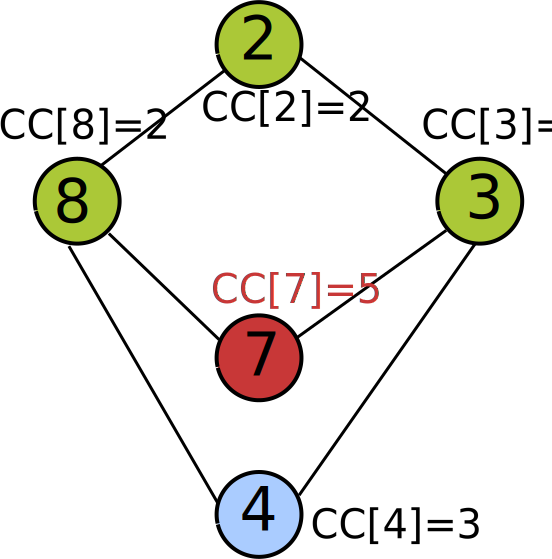
\includegraphics[height=0.5\textheight]{images/fault-corrected/fault-corrected-1}

}
\only<2>{
\centering
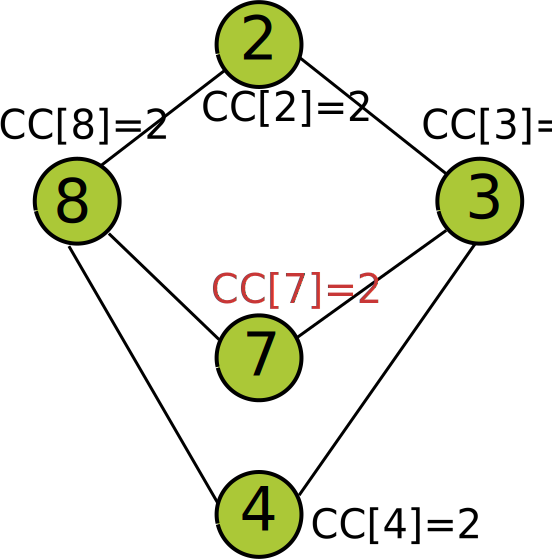
\includegraphics[height=0.5\textheight]{images/fault-corrected/fault-corrected-2}

}
\end{column}
%%%%%%%%%%%% == column == %%%%%%%%%%%%
\begin{column}{0.5\textwidth}
\begin{itemize}
   \item $CC$ value can be corrupted due to hardware faults.
   \item Depending on error caused by the fault, some error can be corrected by the algorithm.
   \item Example: corrupted $CC[v]$ value is arbitrarily high.
   \item Such faults do not cause the algorithm to transition to an invalid state, but they can still cause delay in convergence. 
   \end{itemize}
\end{column}

\end{columns}
\lyxframeend{}

%%%%%%%%%%%%%%%%%%%%%%%%%%%%%%%%%%%%%%%%%%%%%%%%%%%%%%%%%

\lyxframe{Single Fault In Label Propagation Algorithm- Fault Propagation}
\begin{columns}
%%%%%%%%%%%% == column == %%%%%%%%%%%%
\begin{column}{0.5\textwidth}
\only<1>{
\centering
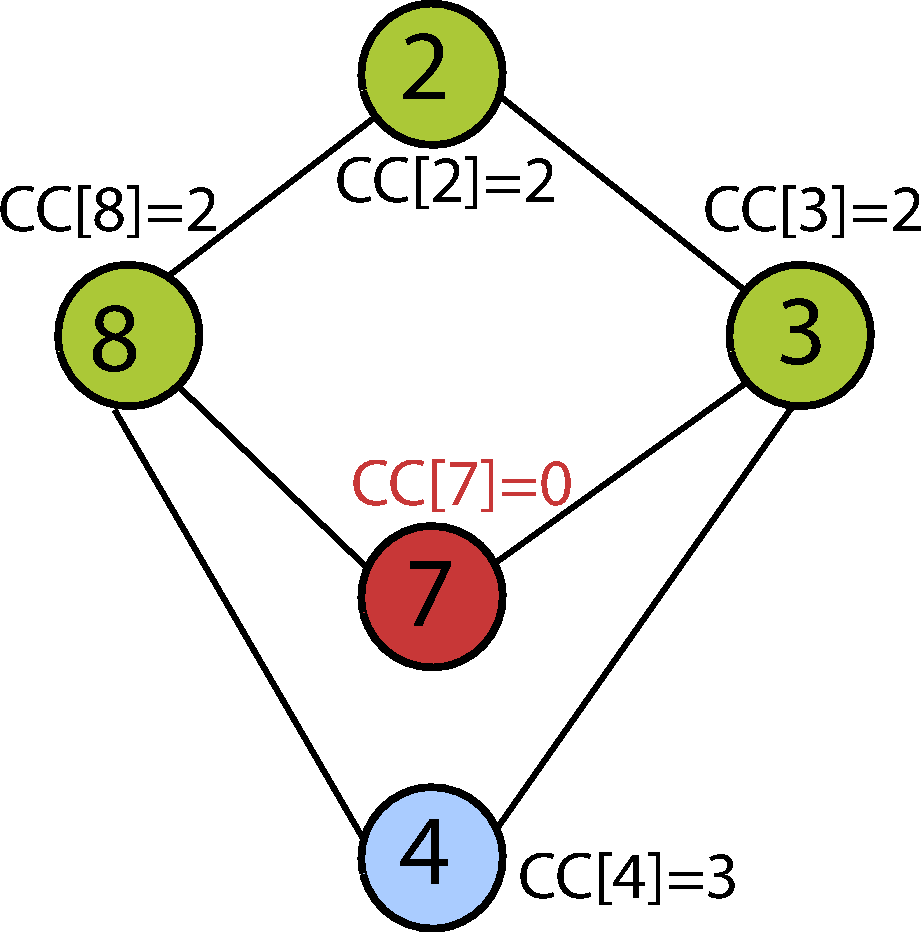
\includegraphics[height=0.5\textheight]{images/fault-propagated/fault-propagated-1}

}
\only<2>{
\centering
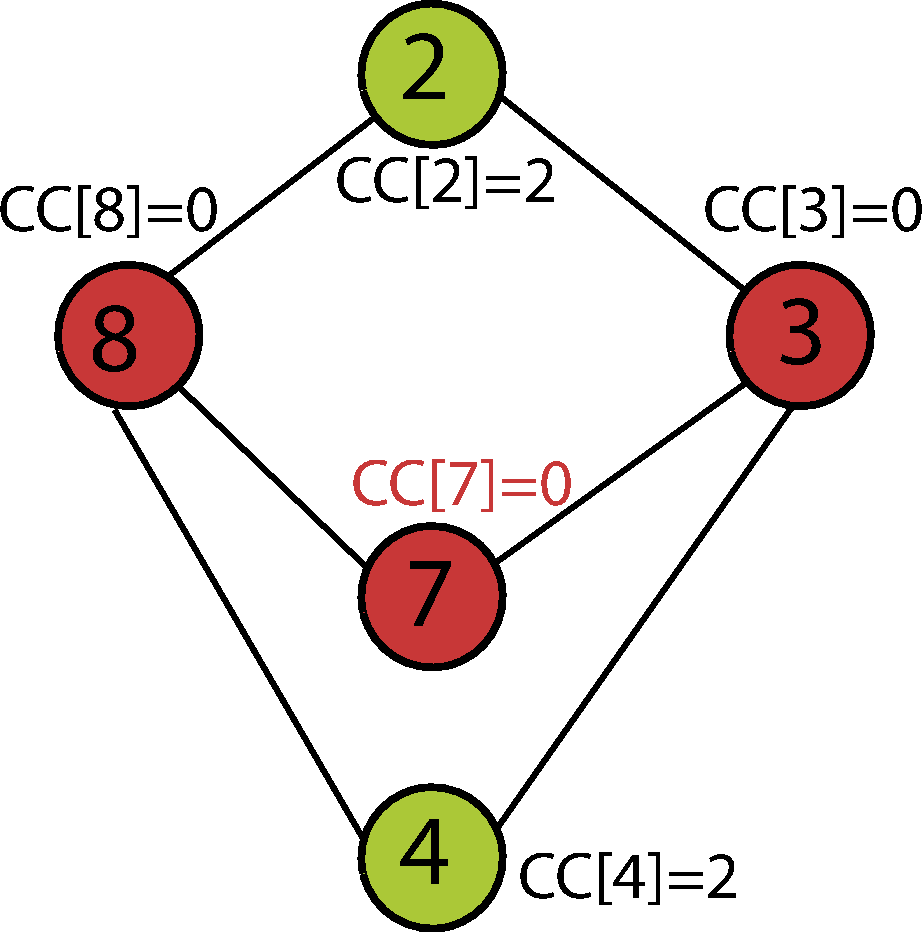
\includegraphics[height=0.5\textheight]{images/fault-propagated/fault-propagated-2}

}
\only<3>{
\centering
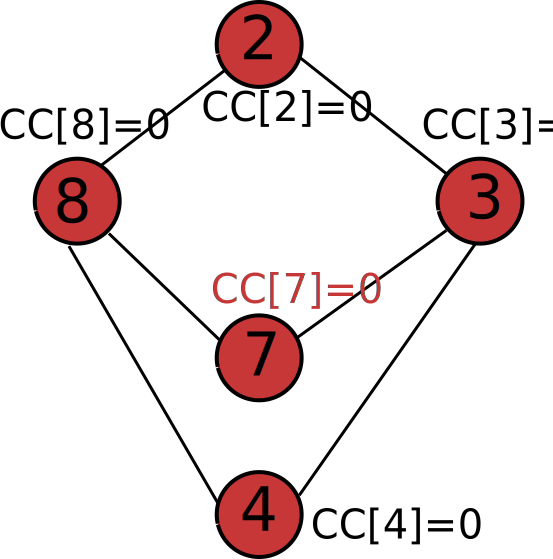
\includegraphics[height=0.5\textheight]{images/fault-propagated/fault-propagated-3}

}
\end{column}
%%%%%%%%%%%% == column == %%%%%%%%%%%%
\begin{column}{0.5\textwidth}
\begin{itemize}
	\item If the fault causes a corruption such $CC[v]$ is changed to a values lower than the $CC^{\infty}[v]$, the error will propagate to all the other vertex in the connected component. 
	\item Such faults do not cause the algorithm to transition to an invalid state.
	\item \color{red} It is not computationally easy to determine whether a given snapshot of $CC$ is a valid state. 
\end{itemize}
\end{column}

\end{columns}
\lyxframeend{}

%%%%%%%%%%%%%%%%%%%%%%%%%%%%%%%%%%%%%%%%%%%%%%%%%%%%%%%%%
\lyxframe{Valid States}
\begin{block}{Classification of different corruption}
Consider following three cases:
\begin{enumerate}
	\item<1-> $CC[v]>v$: Easy to detect and automatically corrected in most cases.  
	\item<2-> $CC^{\infty}[v] \leq CC[v] \leq v$: ??
	\item<3-> {\color{red} $CC[v] < CC^{\infty}[v]$: Will definitely cause algorithm to fail. }
\end{enumerate}
\end{block}


\onslide<4->\begin{theorem}

A connected component array $CC$ is a valid state---i.e.,
a fault-free execution of algorithm  starting from $CC$ will converge to the correct solution---if, for all vertices $v$, 
\[ CC^{\infty}[v] \leq CC[v] \leq v.
\]

\end{theorem} 
% \pause

\onslide<5->
\centering 
\color{red} The only problem is, $CC^{\infty}[v]$---being the solution, is not known. 

\lyxframeend{}
%%%%%%%%%%%%%%%%%%%%%%%%%%%%%%%%%%%%%%%%%%%%%%%%%%%%%%%%%

\lyxframe{Self-correcting Label Propagation Algorithm- 1 }
We apply principle of self-correction to resolve the apparent difficulty in verifying state validity.
\begin{itemize}
\item<2-> We assume the previous state $CC^{i-1}$ is a valid one.
\item<3-> Checking 
\[ CC^{i}[v] = \min_{u \in \mathcal{N}(v)} CC^{i-1}[u], \]
 where  $\mathcal{N}(v) \equiv v \cup adj(v)$ is the immediate \emph{neighborhood} of $v$, {\color{red} will require re-computing entire iteration.}
\item<4-> We show that $CC^{i}[v]$ is still a valid value even if we can relax the minimization criterion to
\[
CC^{i}[v] \in \{ CC^{i-1}[u] \, | \, u \in \mathcal{N}(v) \}, %CC^{i-1}[v]_{adj} \},
\] 

\end{itemize}

\lyxframeend{}

%%%%%%%%%%%%%%%%%%%%%%%%%%%%%%%%%%%%%%%%%%%%%%%%%%%%%%%%%
\lyxframe{Self-correcting Label Propagation Algorithm- 2}
\begin{theorem}
Given a valid state for the previous iteration, $CC^{i-1}$, the current connected component array $CC^{i}$ is a valid state if for all vertices $v$, $CC^{i}$ satisfies these conditions:
\begin{enumerate}
\item $CC^{i}[v] \leq v$; and
\item there exists a vertex $u$ such that $CC^{i}[v]=CC^{i-1}[u]$ and $u \in \mathcal{N}(v)$. %$u \in 
\end{enumerate}
\end{theorem}

\pause
\begin{block}{ Cost of Direct Verification}
\begin{itemize}
\item Verifying $CC^{i}[v] \leq v$ requires $\bigO{V}$ operation.
\item Verifying second condition requires traversing adjacency list for each vertex $v$, that will require
$\bigO{V+E}$ operations, \color{red} as costly as an LP iteration.
\end{itemize}

\end{block}


\lyxframeend{}

%%%%%%%%%%%%%%%%%%%%%%%%%%%%%%%%%%%%%%%%%%%%%%%%%%%%%%%%%
\lyxframe{Validity Checking: Auxiliary Data Structure- 1}
\begin{columns}
%% resize the above figure
\begin{column}{0.5\textwidth}
\only<1>{
\centering
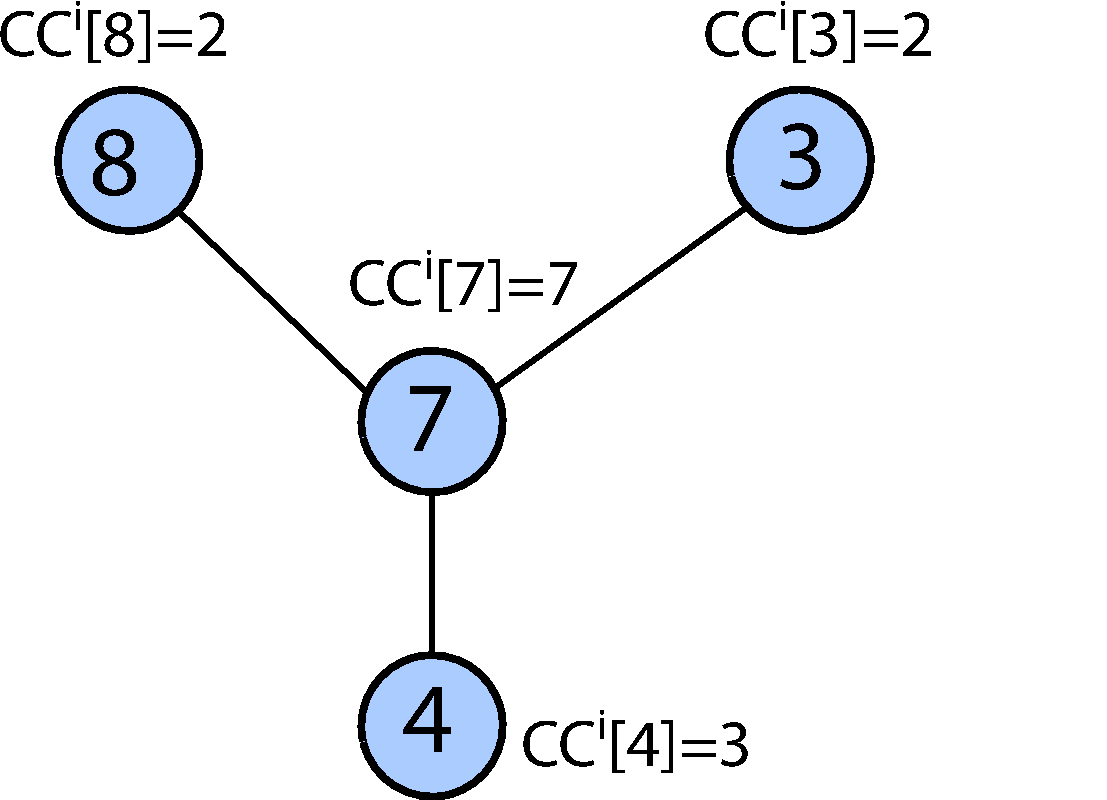
\includegraphics[height=0.5\textheight]{images/parent/parent-1}

}
\only<2->{
\centering
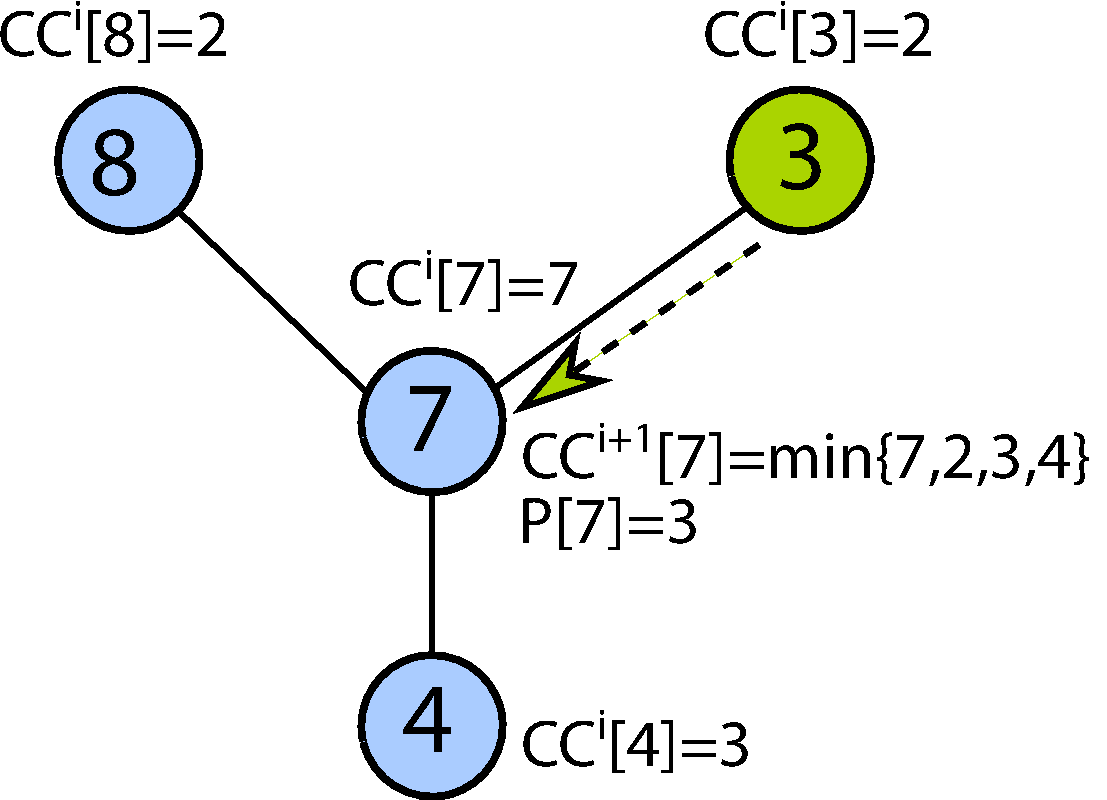
\includegraphics[height=0.5\textheight]{images/parent/parent-2}

}
\end{column}

\begin{column}{0.5\textwidth}
\begin{exampleblock}{Parent Array}
\begin{itemize}
\item Parent array $P$: We may store store information of the vertex $u$ that caused the last change in $CC[v]$.
\item If $u= P[v]$ then $CC^{i}[v] = CC^{i-1}[P[v]]$, can be verified in $\bigO{V}$ operations for all vertex.
\item Storing $P$ requires an memory of $\bigO{V}$.
 \end{itemize}
\end{exampleblock}

\onslide<3->
\begin{alertblock}{Corruption of $P$}

\begin{itemize}
\item $P$ also can be corrupt.
\item $P$ is valid if $P[v] \in \mathcal{N}(v)$ for all vertex $v$.
\item \color{red} Checking $P$ is valid requires again $\bigO{V+E}$ operations.
\end{itemize}
\end{alertblock}
\end{column}
\end{columns}
\lyxframeend{}

%%%%%%%%%%%%%%%%%%%%%%%%%%%%%%%%%%%%%%%%%%%%%%%%%%%%%%%%%
\lyxframe{Validity Checking: Auxiliary Data Structure- 2}
\begin{columns}
\begin{column}{0.5\textwidth}
\centering
\only<1>{
\centering
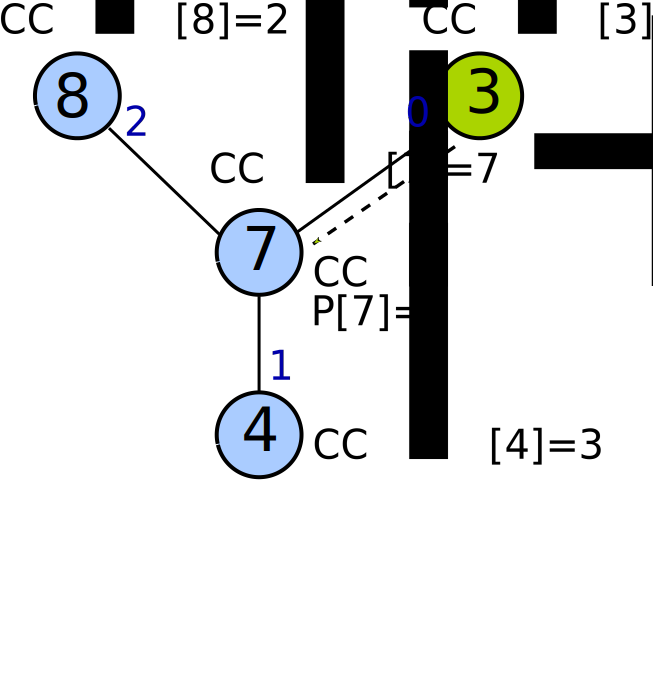
\includegraphics[height=0.5\textheight]{images/parent/new-parent-1}

}
\only<2>{
\centering
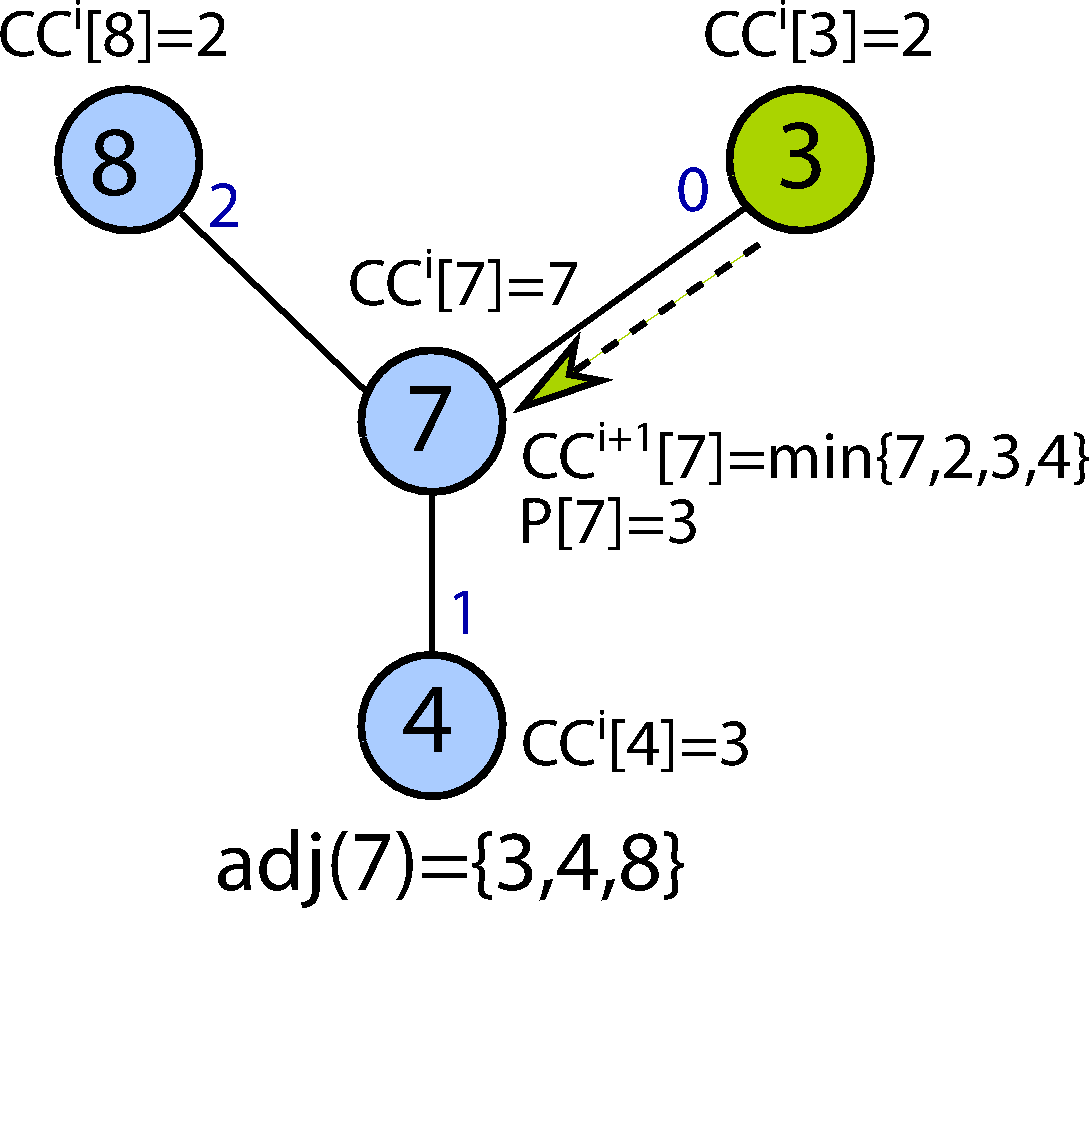
\includegraphics[height=0.5\textheight]{images/parent/new-parent-2}

}
\only<3>{
\centering
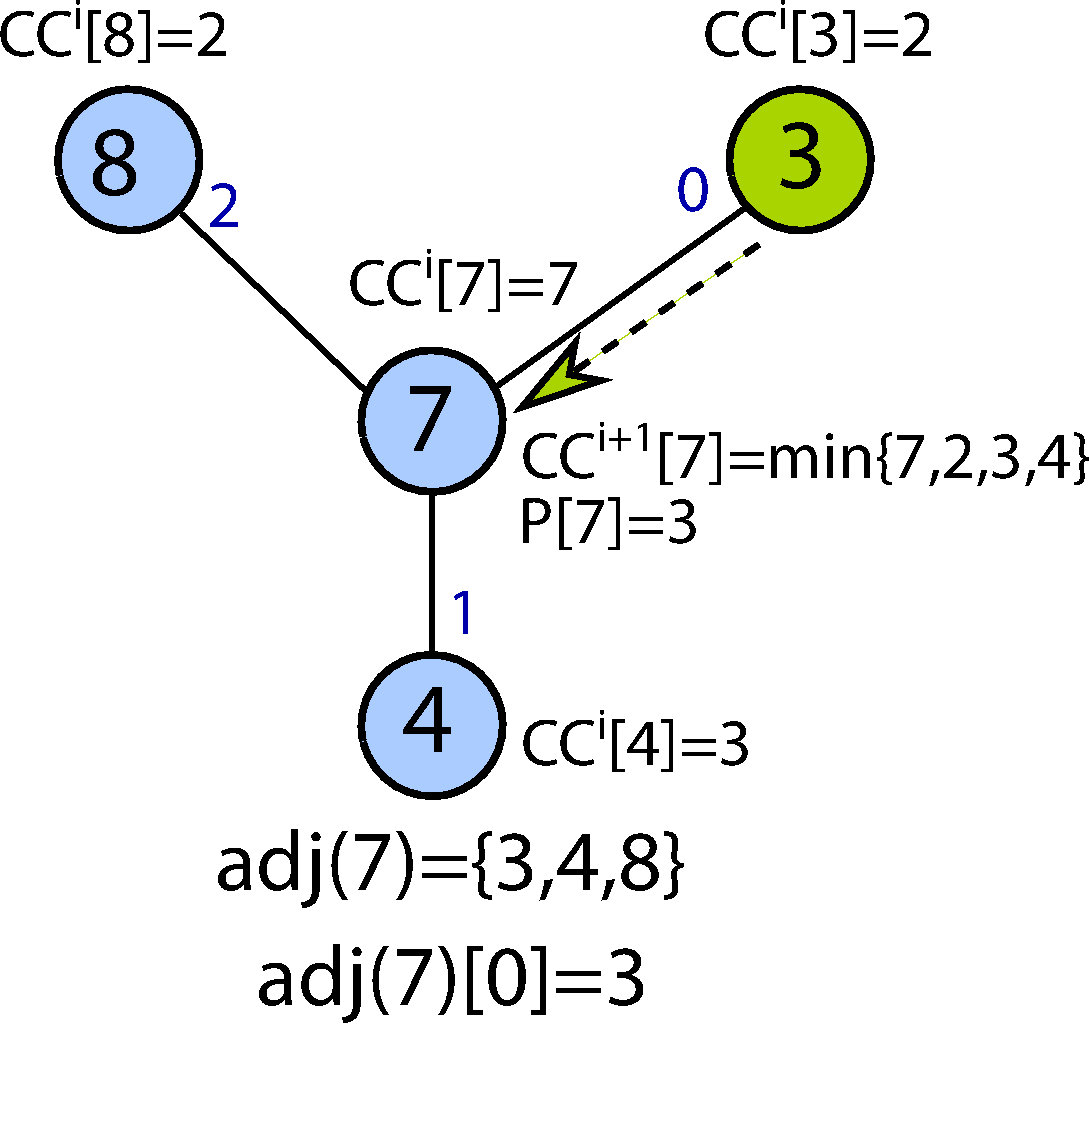
\includegraphics[height=0.5\textheight]{images/parent/new-parent-3}

}
\only<4->{
\centering
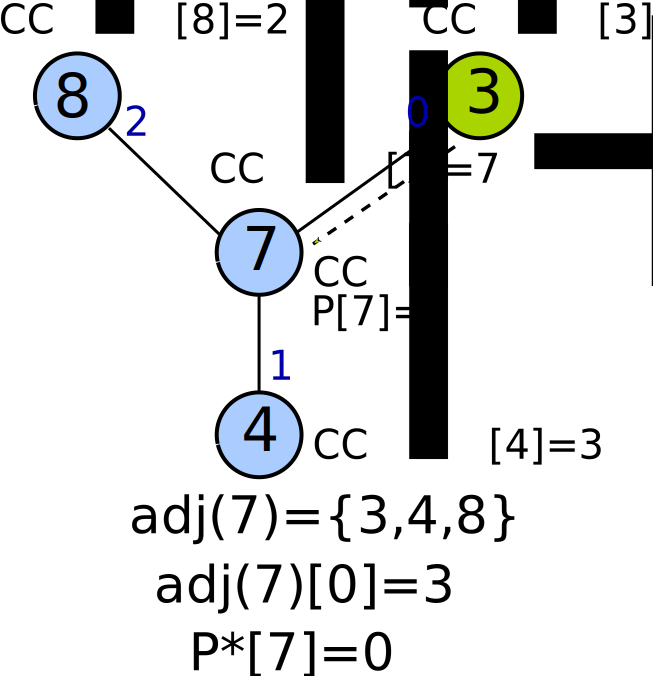
\includegraphics[height=0.5\textheight]{images/parent/new-parent-4}

}
\end{column}
\begin{column}{0.5\textwidth}
\begin{block}{Index Based Parent Array}
\begin{itemize}
\item<1-> Instead of storing $u$, we store index of $u$ in $adj(v)$.
\begin{align*}
       &E & \leftarrow & adj(v) \\
		&u   & \leftarrow & E[k]\\
	&P^{*}[v]   & \leftarrow & k  
\end{align*}
\item<5-> When $P[v]=v$, then  $P^{*}[v]=-1$
\item<6-> $CC^{i}[v] = CC^{i-1}[P[v]]$ reduces to 
\[
	CC^{i}[v] = CC^{i-1}[ adj(v)[P^{*}[v]]];
\]
{\color{dpg} $\bigO{V}$ operations. }% \end{itemize}
% \end{block}

% \begin{block}{}
% \begin{itemize}
% \item $P^{*}$ also requires $\bigO{V}$ memory.
\item<7-> Validity of $P^{*}$:  $-1 \leq P^{*}[v] < |adj(v)| $; 
{\color{dpg}  $\bigO{V}$ operations.}
\end{itemize}
\end{block}
\end{column}
\end{columns}
\lyxframeend{}
%%%%%%%%%%%%%%%%%%%%%%%%%%%%%%%%%%%%%%%%%%%%%%%%%%%%%%%%%

\lyxframe{Fault Detection and Correction}
\begin{exampleblock}{Invalid State Detection}
In summary, the set of conditions to check for each vertex are:
\begin{align*}
\begin{split}
CC^{i}[v] 		&\leq v;  \\
 -1 			&\leq P^{*}[v] < |adj(v)|; \text{and} \\
CC^{i}[v]		&= \begin{cases}
v & \text{ if } P^{*}[v] = -1  \\
CC^{i-1}[ adj(v)[P^{*}[v]]] & \text{ if } P^{*}[v]\ne -1
\end{cases}.
\end{split} 
\end{align*}
\end{exampleblock}

\pause 

\begin{alertblock}{State Correction}
For any vertex $v$, if state validity check fails then, we recompute  $CC^{i}[v]$.
\end{alertblock}
\lyxframeend{}

%%%%%%%%%%%%%%%%%%%%%%%%%%%%%%%%%%%%%%%%%%%%%%%%%%%%%%%%%
\lyxframe{Overhead of Self-correcting Label-propagation Algorithm}
\begin{center}
\begin{tabular}{l|c}
\toprule 
      Overhead           & Asymptotic Complexity     \\
\midrule                  
Fault detection        & $\mathcal{O}(|V|)$      \\
Fault correction       & $\mathcal{O}(f|E|/|V|)$ \\
Auxiliary data structure     & $\mathcal{O}(|V|)$      \\
\bottomrule 
\end{tabular}
\end{center}
\begin{itemize}
\item Number of state corrections $f$, can be significantly less than faults occurred.
\item Fault detection and correction needs to be done in a guaranteed reliable mode.
\end{itemize}

\lyxframeend{}


\section{Self-stabilizing Label-propagation Algorithm}
\lyxframe{Self-stabilizing Connected-component Algorithm- Problem Statement}

\begin{itemize}
\item Given an arbitrary (valid or invalid) state $S={CC,P}$, determine if it is a valid state? 
\item If invalid then construct a valid state $S^{*}$ close to $S={CC,P}$.
\end{itemize}

\lyxframeend{}




\lyxframe{ Parent Tree}

\begin{itemize}
\item Parent Graph $\mathcal{H}$: Subgraph  of $G$ that consists of only edges $(v,P[v])$
\end{itemize}

\lyxframeend{}


\lyxframe{Parent forest}

\begin{itemize}
\item In a fault free execution of label propagation algorithm,  $\mathcal{H}$ is a set of disjoint trees, or \emph{forest}.
\end{itemize}

\lyxframeend{}



\lyxframe{Parent Tree}

\begin{itemize}
\item In a fault free execution, $CC[v]\geq CC[P[v]]$ 
\item If $v$ is a root of a tree, then  $CC[v] = v$ 
\end{itemize}

\lyxframeend{}


\lyxframe{Valid states}

\begin{theorem}

A label propagation state $S=(CC,P)$ is a valid state---i.e.,
a fault-free execution of algorithm  starting from $S$ will converge to the correct solution---if, for all vertices $v$, 

\begin{itemize}
\item $P[v] \in \mathcal{N}(v)$
\item The graph $H=(V, \{\{v,P(v)\}\forall v \in V\} $ does not contain any loops other than self-loops
\item $CC[v] \geq CC[P(v)] $
\end{itemize}

\end{theorem}


\lyxframeend{}



\lyxframe{Verifying Valid states}

\begin{itemize}
\item $P[v] \in \mathcal{N}(v)$ can be done in $\mathcal{O}(V)$
\item $CC[v] \geq CC[v] $  can be done in $\mathcal{O}(V)$
\item The graph $H=(V, \{\{v,P(v)\}\forall v \in V\} $ can be done in $\mathcal{O}(V)$ operation
by using Tarzen's strongly connnected component (SCC) algorithm.
\item Tarzen's strongly connnected component (SCC) is not parallel enough to implement in vertex centric model. 
\end{itemize}

\lyxframeend{}


\lyxframe{Parallel Loop Detection in $\mathcal{H}$ }

\begin{itemize}
\item Calculate $K(v) = \min \{P(v),P{^2}(v), P{^3}(v) \ldots \} $
\end{itemize}

\begin{theorem}
\begin{itemize}
\item If there is no loop, then $K(v) < v$ for all $v$ except for the root of a tree. 
\item If $K(v)=v$, then there is a loop, and $v$ has minimum vertex id among all the element in the loop. 
\end{itemize}
\end{theorem}

\lyxframeend{}


\lyxframe{Calculating $K(v) = \min \{P(v),P{^2}(v), P{^3}(v) \ldots \}$ }

\begin{itemize}
\item Calculating  $K(v)$ is a \emph{prefix} sum operation.
\item Initialize: $K(v) = P(v)$
\item Update: $K(v) = \min \{ K(v), P(K(v)) \}$
\item Terminate when no $K(v)$ changes. 
\end{itemize}

\begin{itemize}
\item Cost $\mathcal{O}(V \log V)$
\end{itemize}

\lyxframeend{}

\lyxframe{ Verifying Valid  of a State}

\begin{itemize}
\item $P[v] \in \mathcal{N}(v)$
\item The graph $H=(V, \{\{v,P(v)\}\forall v \in V\} $ does not contain any loops other than self-loops
\item $CC[v] \geq CC[P(v)] $ (Not needed)
\end{itemize}


\lyxframeend{}


\lyxframe{ State Correction}
Hyatt Place Albuquer Uptown
\begin{itemize}
\item $P[v] \notin \mathcal{N}(v)$, reset $v$, $CC[v]=v$, $P(v)=v$
\item Calculate $K(v)$. If $K(v)=v$, break the loop at $v$, $P(v)=v$.
\item Set $CC[v] = K(v)$.
\end{itemize}


\begin{itemize}
\item Previosuly used periodic correction scheme to bring it to a valid state.
\item Often Label propagation algorithm takes very few iteration to converge.
\item We perform correction step only once at the end of label propagation.
\end{itemize}

\lyxframeend{}


\lyxframe{ A Practical Fault Tolerant Label-propagation algorithm}

\begin{itemize}
\item Frequently 2-loops are formed. 
\item Slows down the convergence.
\end{itemize}


\begin{itemize}
\item In every iteration, we perform some checks to stop fault propagation.
\begin{enumerate}
	\item $P(v) \in \mathcal{N}(v)$
	\item $CC[v] \geq CC[p(v)]$
	\item Two loop detection: $v = P(P(v))$.
\end{enumerate} 


\item Cost $\mathcal{O}(V)$ 
\item These checks can be unreliable.
\end{itemize}

\lyxframeend{}


\lyxframe{ To summerize }

\begin{itemize}
\item Requires additional O(v) memory
\item Costs log(v)
\item May take additional iterations.
\end{itemize}

\lyxframeend{}



\section{Experiments and Results}
\lyxframe{Experimental Setup }

\begin{block}{Machine Parameter}
\begin{center}
\begin{tabular}{l|l}
\toprule
Prop                 & SNB16c       \\
\midrule
Micro-architecture    & Sandy-Bridge  \\
Sockets$\times$Cores & 2$\times$8   \\
Clock Rate           & 2.4GHz       \\
DRAM capacity        & 128GB        \\
DRAM Bandwidth       & 72GB/s      \\
Compiler       		 & Intel ``C'' compiler 15.0.0     \\
\bottomrule
\end{tabular}
\end{center}
\end{block}

\begin{block}{Fault Injection}
\begin{itemize}
\item Fault injection in reading graph data structure and $CC$ array.
\item Each fault injection read is independent
\item Normalized by number of edges in the network
\end{itemize}
\end{block}

\begin{itemize}
\item Test Network: $14^{th}$ DIMACS graph challenge
\end{itemize}
\lyxframeend{}

%%%%%%%%%%%%%%%%%%%%%%%%%%%%%%%%%%%%%%%%%%%%%%%%%%%%%%%%%

\lyxframe{Fault Free Execution Overhead }
\centering
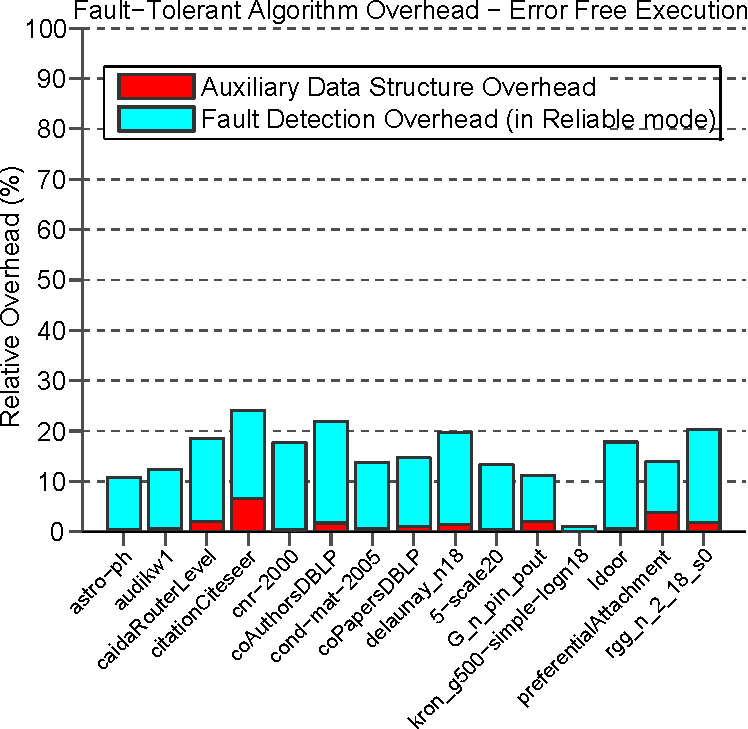
\includegraphics[height=.75\textheight]{plots/plot_zero_overhead-1}

\color{dpg} On an average 1.3\% overhead for maintaining additional data structure and 14\%
for fault detection.
\lyxframeend{}

%%%%%%%%%%%%%%%%%%%%%%%%%%%%%%%%%%%%%%%%%%%%%%%%%%%%%%%%%
\lyxframe{Failure Rate for synchronous case }
\centering
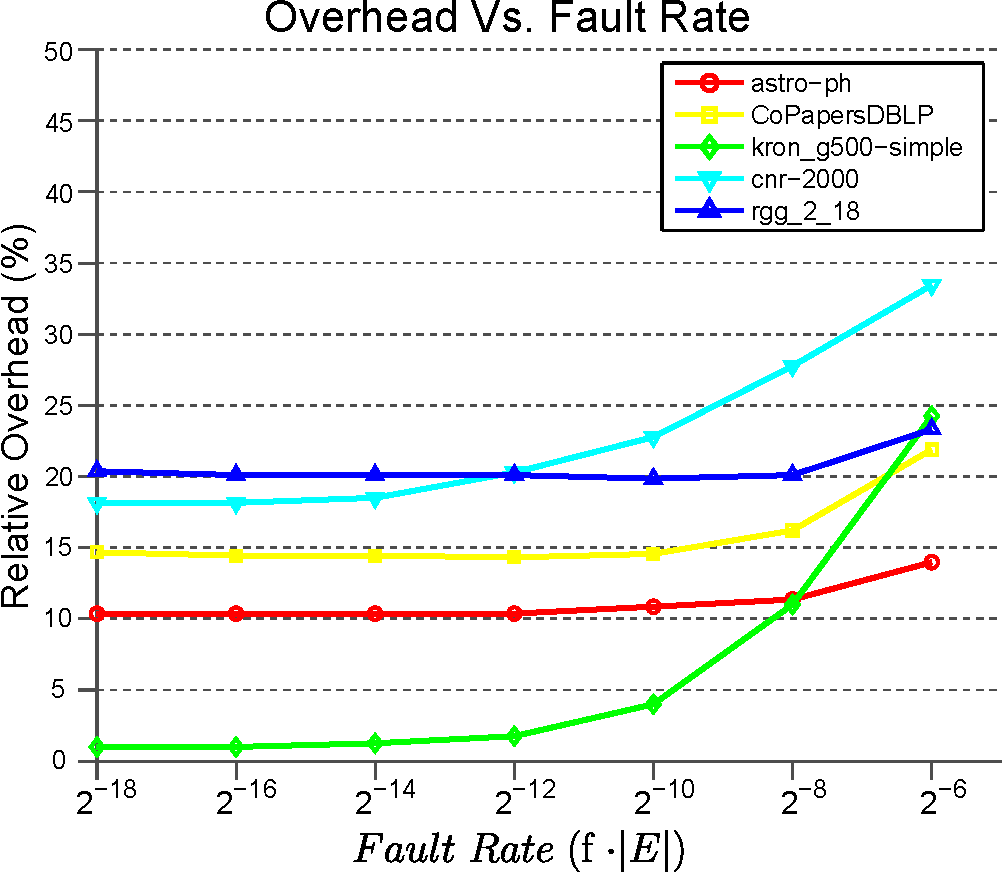
\includegraphics[height=.75\textheight]{plots/plot_overhead_fault-inked}

\lyxframeend{}
%%%%%%%%%%%%%%%%%%%%%%%%%%%%%%%%%%%%%%%%%%%%%%%%%%%%%%%%%


%%%%%%%%%%%%%%%%%%%%%%%%%%%%%%%%%%%%%%%%%%%%%%%%%%%%%%%%%
\lyxframe{Fault free overhead }
\centering
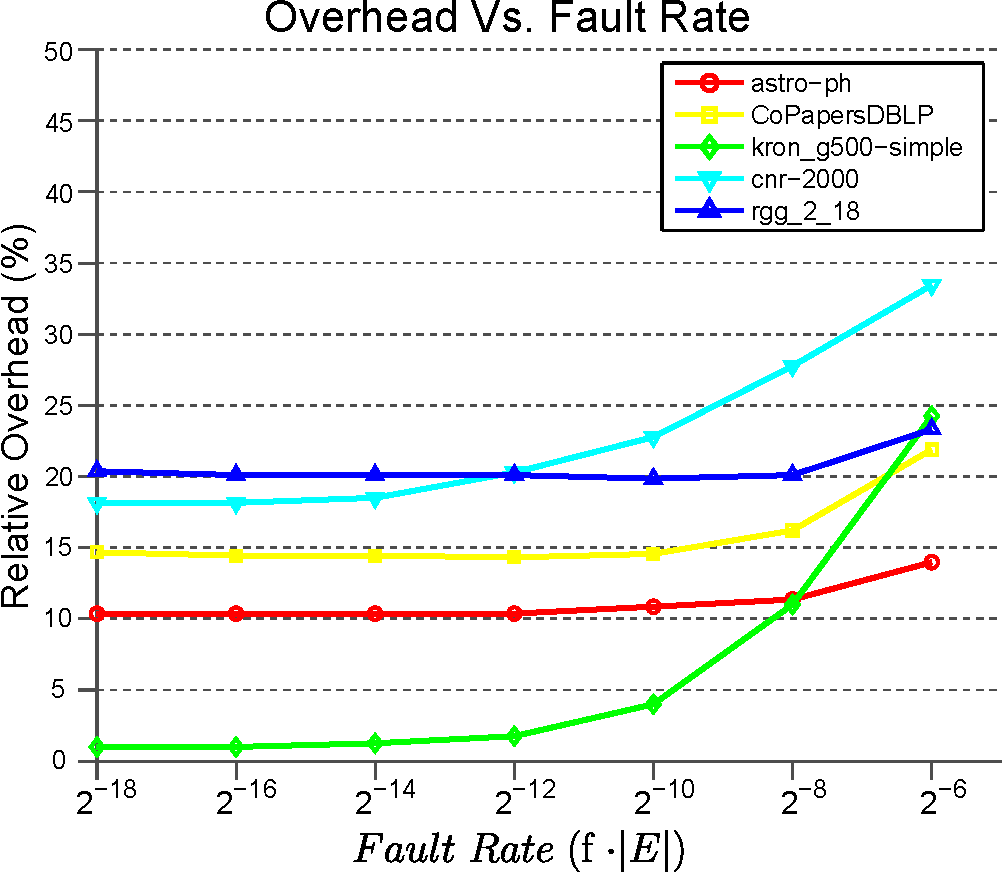
\includegraphics[height=.75\textheight]{plots/plot_overhead_fault-inked}

\lyxframeend{}
%%%%%%%%%%%%%%%%%%%%%%%%%%%%%%%%%%%%%%%%%%%%%%%%%%%%%%%%%

%%%%%%%%%%%%%%%%%%%%%%%%%%%%%%%%%%%%%%%%%%%%%%%%%%%%%%%%%
\lyxframe{Failure Rate for asynchronous case }
\centering
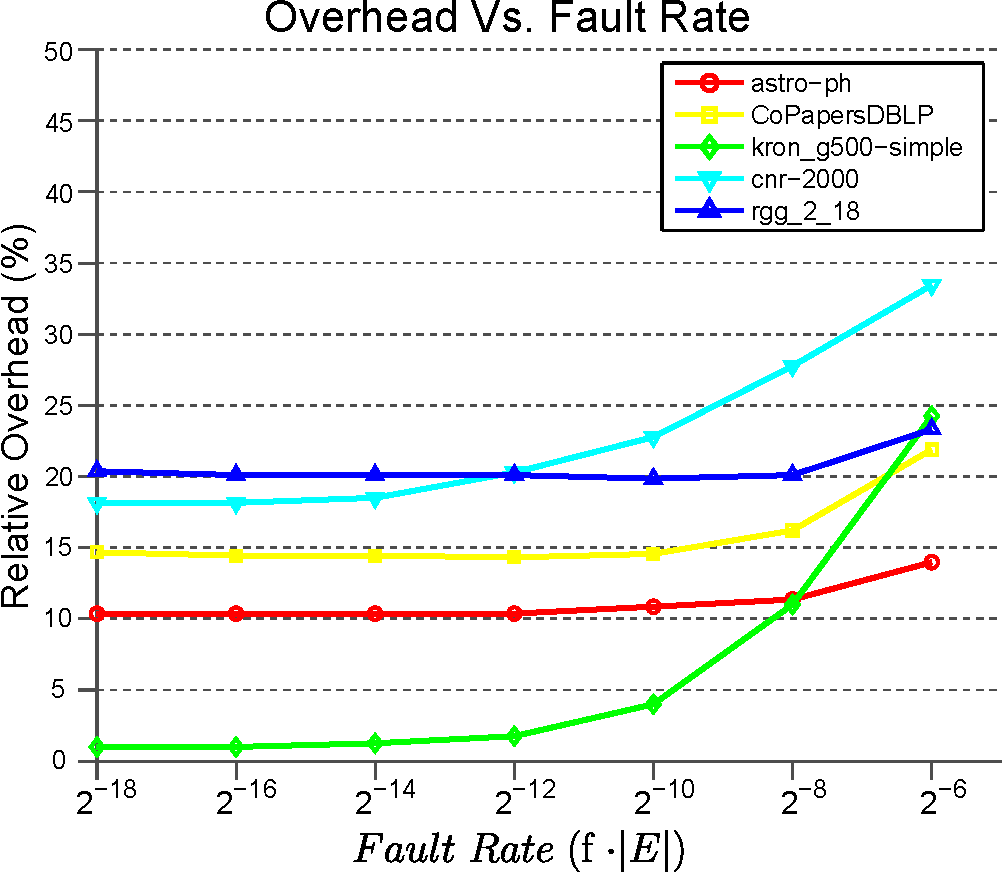
\includegraphics[height=.75\textheight]{plots/plot_overhead_fault-inked}

\lyxframeend{}
%%%%%%%%%%%%%%%%%%%%%%%%%%%%%%%%%%%%%%%%%%%%%%%%%%%%%%%%%


%%%%%%%%%%%%%%%%%%%%%%%%%%%%%%%%%%%%%%%%%%%%%%%%%%%%%%%%%
\lyxframe{Histogram for convergence}
\centering
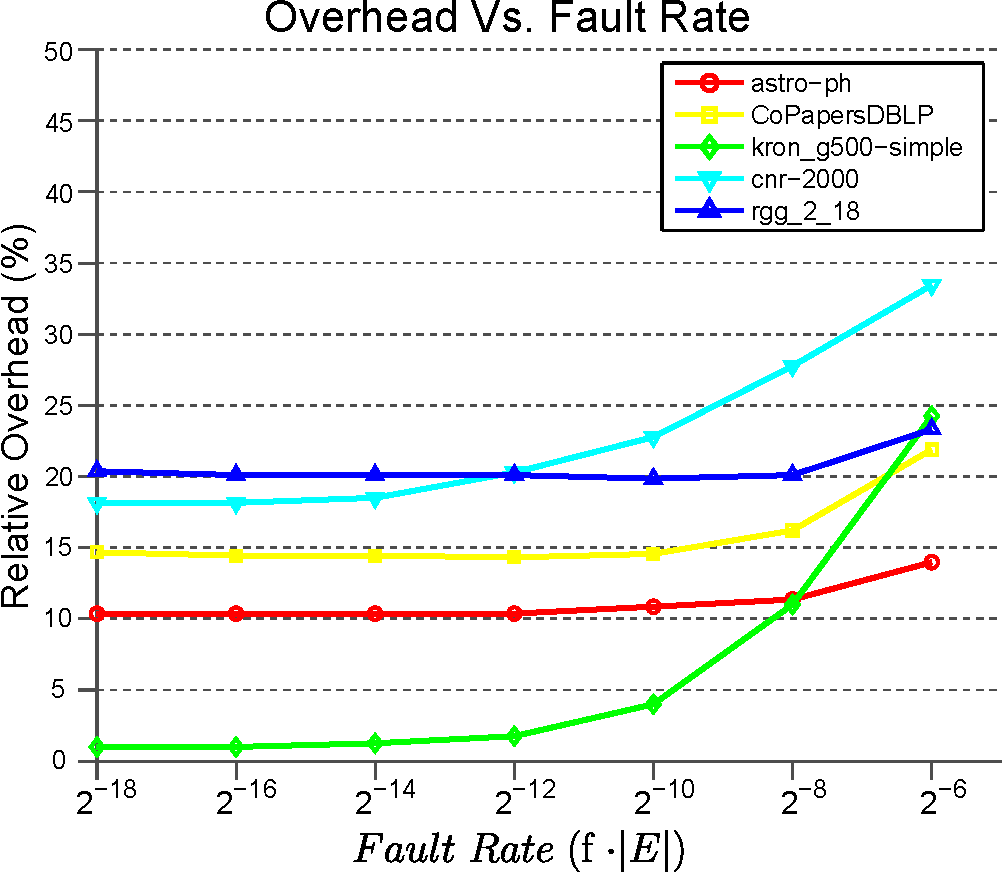
\includegraphics[height=.75\textheight]{plots/plot_overhead_fault-inked}
\lyxframeend{}
%%%%%%%%%%%%%%%%%%%%%%%%%%%%%%%%%%%%%%%%%%%%%%%%%%%%%%%%%



\section{Conclusion}
\textbf{\emph{c}}\emph{onlusion} 
\begin{itemize}
\item what did we do 
\item what are implications 
\item where do we go from here 
\end{itemize}



% \section{Introduction}
% 

The exceeding growth of big datasets has created a need for using distributed systems and 
accelerators for real-time analytics, including for graph and social network analytics. Social 
networks such Facebook and Twitter are constantly growing  at time of writing have over #### 
members with **** relationships between these members.
The decrease of transistor sizes and the improved power consumption, as part of Moore's laws, has 
brought a new challenge with it - an increased number of faults due to random bit flipping. This 
problem is very likely to become even more challenging as transistor sizes continue to decrease and 
the power envelope restrictions become even tighter. As larger systems, with a higher thread count, 
become ubiquitous so will the problem of power related faults.

In this work, we tackle the problem of faults in a connected component algorithm that is 
propagation based. We modify the parallel algorithm of Shiloach-Vishkin \cite{shiloachvishkin} and 
make it fault-tolerant by augmenting the data structures used by the algorithm and by adding a 
detection and correction scheme at the end of every iteration. By detecting and correcting the 
error at the end of each iteration we are able to limit the propagation of the error to the 
remainder of the graph in the following iterations.

Main contributions:
* Little overhead when there aren't any faults.
* Same number of iterations as a fault-free execution for reasonable error rates.
* Overhead if rather constant in time until the number of threads is significantly high.
* 




% \section{HALO Algorithm}
% \input{halo}

% \section{Overcoming Limited Memory of Co-processor}
% \input{limited_mem}
% \section{Experiments and Results}
% \lyxframe{Experimental Setup }

\begin{block}{Machine Parameter}
\begin{center}
\begin{tabular}{l|l}
\toprule
Prop                 & SNB16c       \\
\midrule
Micro-architecture    & Sandy-Bridge  \\
Sockets$\times$Cores & 2$\times$8   \\
Clock Rate           & 2.4GHz       \\
DRAM capacity        & 128GB        \\
DRAM Bandwidth       & 72GB/s      \\
Compiler       		 & Intel ``C'' compiler 15.0.0     \\
\bottomrule
\end{tabular}
\end{center}
\end{block}

\begin{block}{Fault Injection}
\begin{itemize}
\item Fault injection in reading graph data structure and $CC$ array.
\item Each fault injection read is independent
\item Normalized by number of edges in the network
\end{itemize}
\end{block}

\begin{itemize}
\item Test Network: $14^{th}$ DIMACS graph challenge
\end{itemize}
\lyxframeend{}

%%%%%%%%%%%%%%%%%%%%%%%%%%%%%%%%%%%%%%%%%%%%%%%%%%%%%%%%%

\lyxframe{Fault Free Execution Overhead }
\centering
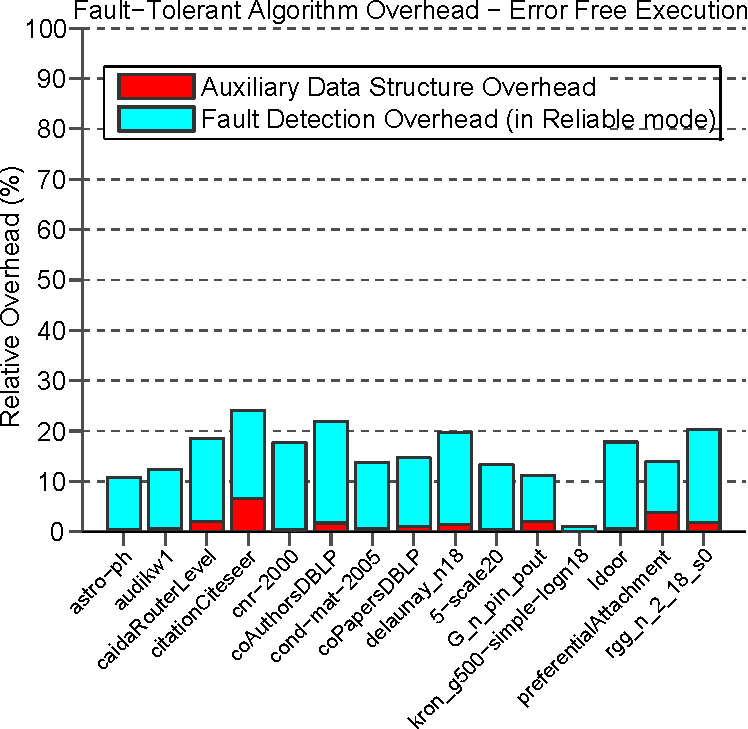
\includegraphics[height=.75\textheight]{plots/plot_zero_overhead-1}

\color{dpg} On an average 1.3\% overhead for maintaining additional data structure and 14\%
for fault detection.
\lyxframeend{}

%%%%%%%%%%%%%%%%%%%%%%%%%%%%%%%%%%%%%%%%%%%%%%%%%%%%%%%%%
\lyxframe{Failure Rate for synchronous case }
\centering
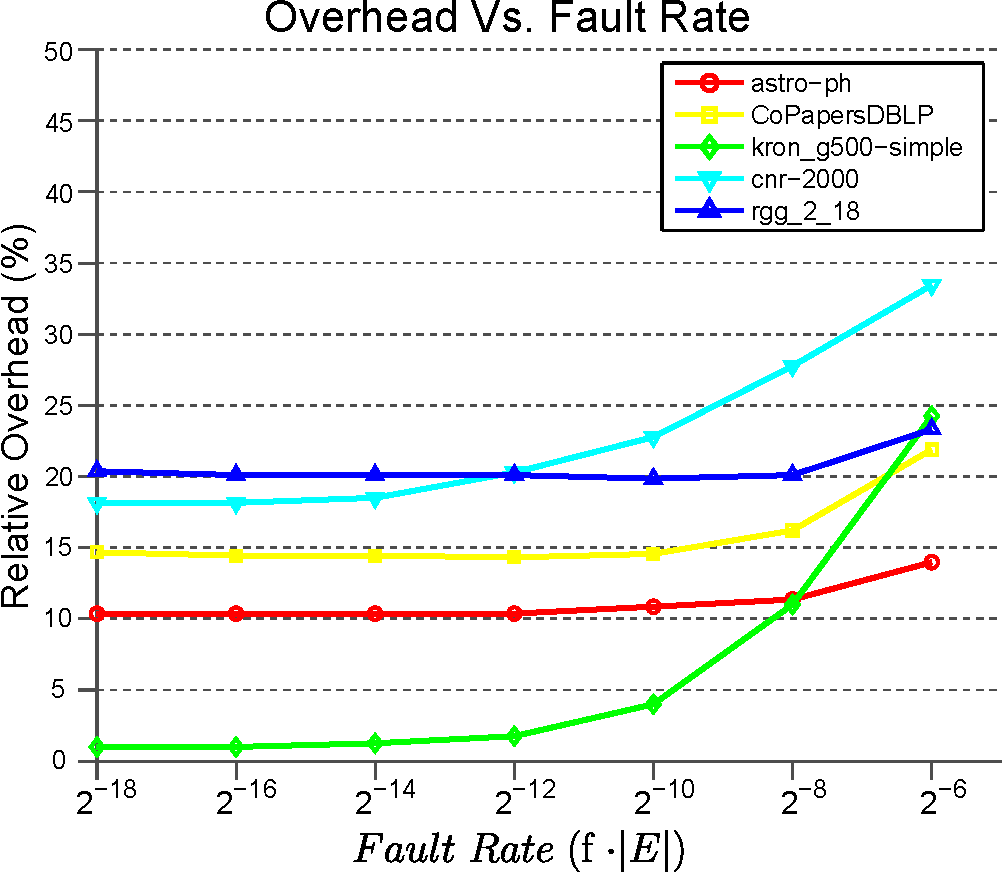
\includegraphics[height=.75\textheight]{plots/plot_overhead_fault-inked}

\lyxframeend{}
%%%%%%%%%%%%%%%%%%%%%%%%%%%%%%%%%%%%%%%%%%%%%%%%%%%%%%%%%


%%%%%%%%%%%%%%%%%%%%%%%%%%%%%%%%%%%%%%%%%%%%%%%%%%%%%%%%%
\lyxframe{Fault free overhead }
\centering
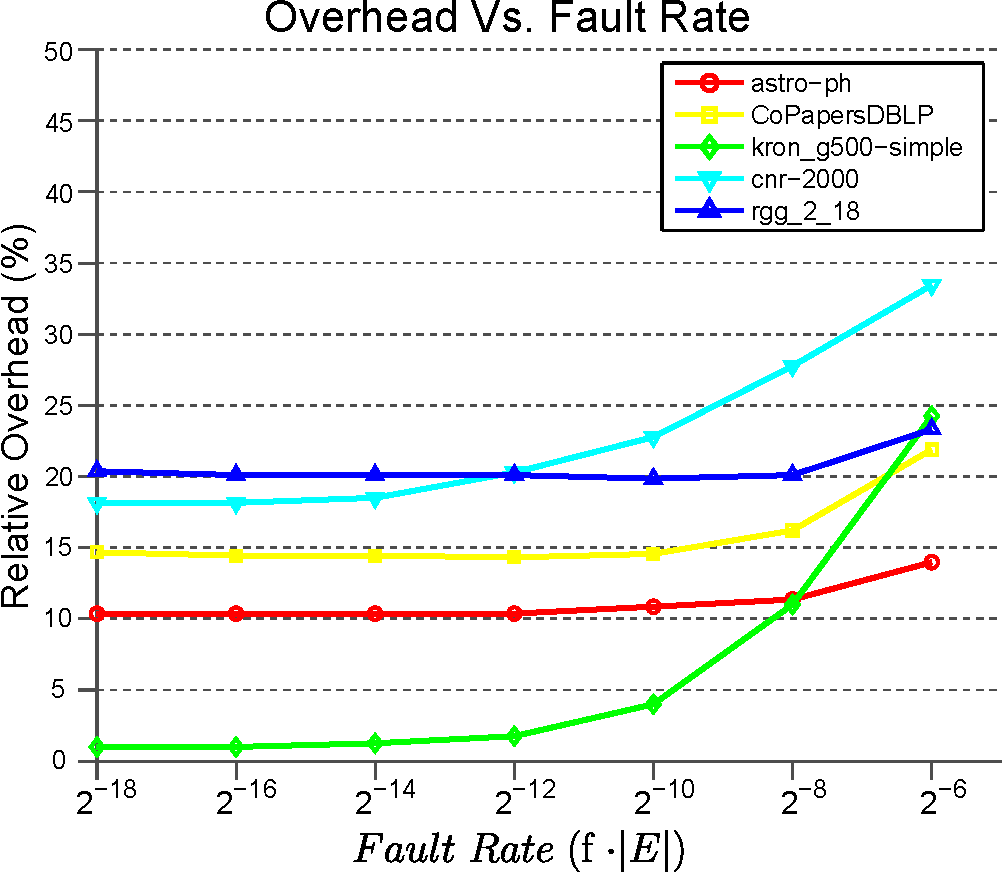
\includegraphics[height=.75\textheight]{plots/plot_overhead_fault-inked}

\lyxframeend{}
%%%%%%%%%%%%%%%%%%%%%%%%%%%%%%%%%%%%%%%%%%%%%%%%%%%%%%%%%

%%%%%%%%%%%%%%%%%%%%%%%%%%%%%%%%%%%%%%%%%%%%%%%%%%%%%%%%%
\lyxframe{Failure Rate for asynchronous case }
\centering
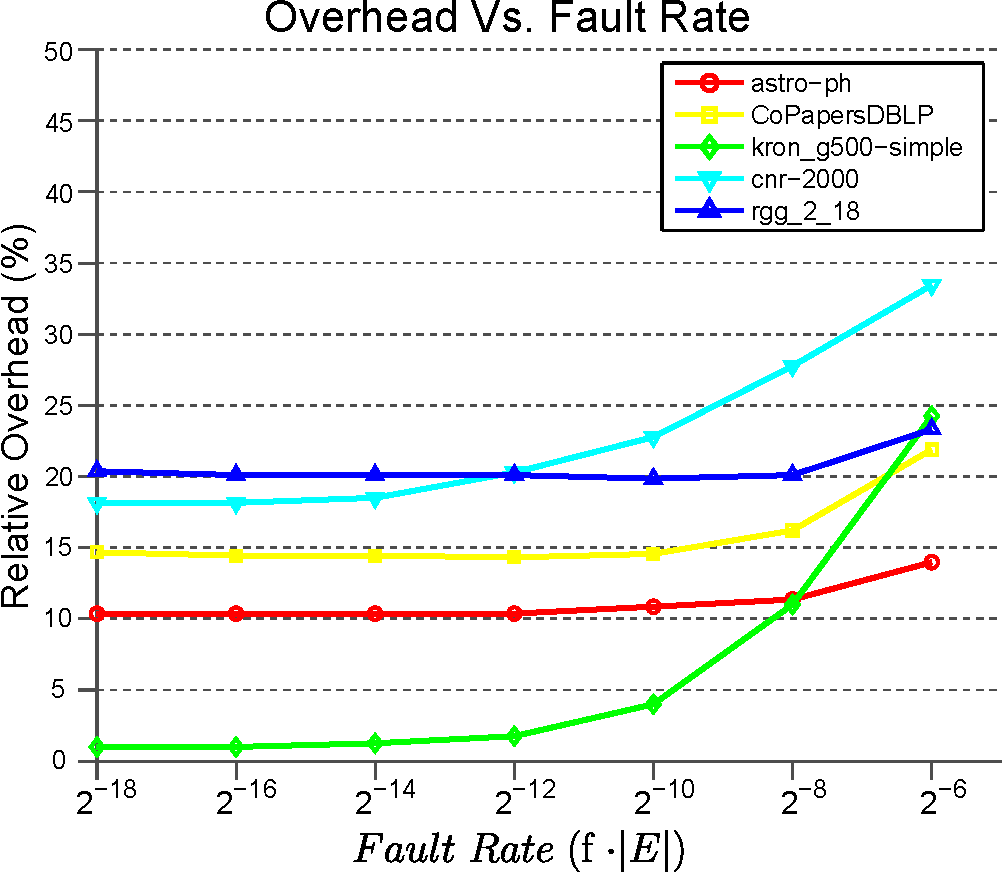
\includegraphics[height=.75\textheight]{plots/plot_overhead_fault-inked}

\lyxframeend{}
%%%%%%%%%%%%%%%%%%%%%%%%%%%%%%%%%%%%%%%%%%%%%%%%%%%%%%%%%


%%%%%%%%%%%%%%%%%%%%%%%%%%%%%%%%%%%%%%%%%%%%%%%%%%%%%%%%%
\lyxframe{Histogram for convergence}
\centering
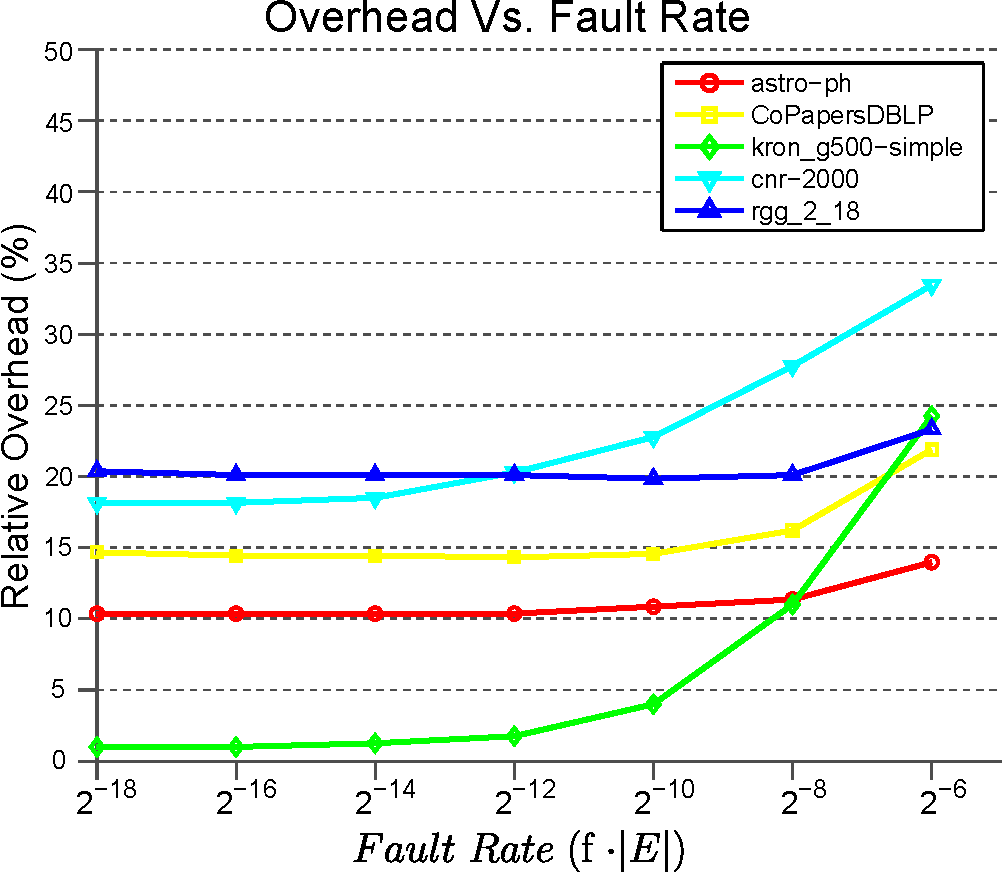
\includegraphics[height=.75\textheight]{plots/plot_overhead_fault-inked}
\lyxframeend{}
%%%%%%%%%%%%%%%%%%%%%%%%%%%%%%%%%%%%%%%%%%%%%%%%%%%%%%%%%



% \section{Conclusion}
% \textbf{\emph{c}}\emph{onlusion} 
\begin{itemize}
\item what did we do 
\item what are implications 
\item where do we go from here 
\end{itemize}



% \section{Intranode Load Balance}
% \input{intranode-loadbalance}


\end{document}
